\documentclass[a4paper, 11pt]{article}
\usepackage{comment} % enables the use of multi-line comments (\ifx \fi) 
\usepackage{fullpage}
\usepackage{geometry}
\usepackage{amsmath}
\usepackage{amssymb}
\usepackage{gensymb}
\usepackage{listings}
\renewcommand{\lstlistingname}{Code}
\usepackage[labelfont=bf]{caption}
\usepackage{graphicx}
\usepackage{epstopdf}
\usepackage{subcaption}
\usepackage{multirow}
\usepackage{hhline}
\usepackage{bm}
\usepackage{rotfloat}
\usepackage[most]{tcolorbox}
\usepackage{inconsolata}
\newtcblisting[auto counter]{code}[2][]{
    fonttitle=\bfseries, colframe=gray, listing only, 
    listing options={basicstyle=\ttfamily,language=C}, 
    title=Code \thetcbcounter: #2, #1}
\newtcblisting[auto counter]{algorithm}[2][]{
    fonttitle=\bfseries, colframe=gray, listing only, 
    listing options={basicstyle=\small, mathescape, }, 
    title=Algorithm \thetcbcounter: #2, #1}
\lstset{numbers=left, numberstyle=\tiny, stepnumber=1, numbersep=5pt, tabsize=3}
\usepackage{tikz}
\usetikzlibrary{shapes,arrows,positioning,calc}
% \makeatletter
% \renewcommand\thesection{}
% \renewcommand\thesubsection{\@arabic\c@section.\@arabic\c@subsection}
% \makeatother


\begin{document}

%% LIS Report Header Template
%%%%%%%%%%%%%%%%%%%%%%%%%%%%%%%%%%%%%%%%%%%%%%%%%%%%%%%%%%%%%

%%%%%%%%%%%%%%%%%%%%%%%%%%%%%%%%%%%%%%%%%%%%%%%%%%%%%%%%%%%%%
%% 
%%%%%%%%%%%%%%%%%%%%%%%%%%%%%%%%%%%%%%%%%%%%%%%%%%%%%%%%%%%%%
%%
%% ATTENTION: You need a main file to use this one here.
%%            Use the command "%% LIS Report Header Template
%%%%%%%%%%%%%%%%%%%%%%%%%%%%%%%%%%%%%%%%%%%%%%%%%%%%%%%%%%%%%

%%%%%%%%%%%%%%%%%%%%%%%%%%%%%%%%%%%%%%%%%%%%%%%%%%%%%%%%%%%%%
%% 
%%%%%%%%%%%%%%%%%%%%%%%%%%%%%%%%%%%%%%%%%%%%%%%%%%%%%%%%%%%%%
%%
%% ATTENTION: You need a main file to use this one here.
%%            Use the command "%% LIS Report Header Template
%%%%%%%%%%%%%%%%%%%%%%%%%%%%%%%%%%%%%%%%%%%%%%%%%%%%%%%%%%%%%

%%%%%%%%%%%%%%%%%%%%%%%%%%%%%%%%%%%%%%%%%%%%%%%%%%%%%%%%%%%%%
%% 
%%%%%%%%%%%%%%%%%%%%%%%%%%%%%%%%%%%%%%%%%%%%%%%%%%%%%%%%%%%%%
%%
%% ATTENTION: You need a main file to use this one here.
%%            Use the command "\input{titlepage}" in your
%%            main file to include this file.
%%

%%%%%%%%%%%%%%%%%%%%%%%%%%%%%%%%%%%%%%%%%%%%%%%%%%
%% Macros that are filled into the standard text:

%% Things that change for each project:
\newcommand{\Ptype}{Semester Project} %DIPLOMA
\newcommand{\Ptitle}{Optic-Flow based estimation of angle of attack}
\newcommand{\Pcand}{Brice Platerrier}
\newcommand{\Psect}{Section Microtechnique}
\newcommand{\Pprof}{Dario Floreano}
\newcommand{\Pfirst}{Julien Lecoeur}
\newcommand{\Psecond}{}
%% Dates that depend only on the semester:
\newcommand{\Pseason}{FEBRUARY 2015 / 2016} %put here the semester name



\begin{titlepage}

\begin{center}


\includegraphics[width=4cm]{logo_epfl_coul.eps}

%\vspace*{1cm}
\vspace*{5cm}
\Large
\textsc{\Ptitle}\\
\vspace{0.5cm}
\normalsize
\textsc{\Ptype }\\ %semster 
\vspace{1.5cm}

%\LARGE
\large
%von
\textsc{\Pcand\\[0.5\baselineskip] }
\normalsize
\textsc{\Psect}\\
%{ born on the 26th of April 1994 in Toulouse, France}}}\\
\vspace{1cm}

\textsc{\Pseason}\\ %%Date - better you write it yourself.
\vspace{2cm}
\textsc{Assistants:\\ \Pfirst}\\
\vspace{1cm}
\textsc{Laboratory of Intelligent Systems (LIS)\\
Prof. \Pprof\\}


\vspace{1.5cm}
\textsc{EPFL\\
Faculte Sciences et Techniques de l'ingenieur (STI)\\
Institut d'ingenierie des systemes (I2S) }\\

\end{center}

\end{titlepage}
" in your
%%            main file to include this file.
%%

%%%%%%%%%%%%%%%%%%%%%%%%%%%%%%%%%%%%%%%%%%%%%%%%%%
%% Macros that are filled into the standard text:

%% Things that change for each project:
\newcommand{\Ptype}{Semester Project} %DIPLOMA
\newcommand{\Ptitle}{Optic-Flow based estimation of angle of attack}
\newcommand{\Pcand}{Brice Platerrier}
\newcommand{\Psect}{Section Microtechnique}
\newcommand{\Pprof}{Dario Floreano}
\newcommand{\Pfirst}{Julien Lecoeur}
\newcommand{\Psecond}{}
%% Dates that depend only on the semester:
\newcommand{\Pseason}{FEBRUARY 2015 / 2016} %put here the semester name



\begin{titlepage}

\begin{center}


\includegraphics[width=4cm]{logo_epfl_coul.eps}

%\vspace*{1cm}
\vspace*{5cm}
\Large
\textsc{\Ptitle}\\
\vspace{0.5cm}
\normalsize
\textsc{\Ptype }\\ %semster 
\vspace{1.5cm}

%\LARGE
\large
%von
\textsc{\Pcand\\[0.5\baselineskip] }
\normalsize
\textsc{\Psect}\\
%{ born on the 26th of April 1994 in Toulouse, France}}}\\
\vspace{1cm}

\textsc{\Pseason}\\ %%Date - better you write it yourself.
\vspace{2cm}
\textsc{Assistants:\\ \Pfirst}\\
\vspace{1cm}
\textsc{Laboratory of Intelligent Systems (LIS)\\
Prof. \Pprof\\}


\vspace{1.5cm}
\textsc{EPFL\\
Faculte Sciences et Techniques de l'ingenieur (STI)\\
Institut d'ingenierie des systemes (I2S) }\\

\end{center}

\end{titlepage}
" in your
%%            main file to include this file.
%%

%%%%%%%%%%%%%%%%%%%%%%%%%%%%%%%%%%%%%%%%%%%%%%%%%%
%% Macros that are filled into the standard text:

%% Things that change for each project:
\newcommand{\Ptype}{Semester Project} %DIPLOMA
\newcommand{\Ptitle}{Optic-Flow based estimation of angle of attack}
\newcommand{\Pcand}{Brice Platerrier}
\newcommand{\Psect}{Section Microtechnique}
\newcommand{\Pprof}{Dario Floreano}
\newcommand{\Pfirst}{Julien Lecoeur}
\newcommand{\Psecond}{}
%% Dates that depend only on the semester:
\newcommand{\Pseason}{FEBRUARY 2015 / 2016} %put here the semester name



\begin{titlepage}

\begin{center}


\includegraphics[width=4cm]{logo_epfl_coul.eps}

%\vspace*{1cm}
\vspace*{5cm}
\Large
\textsc{\Ptitle}\\
\vspace{0.5cm}
\normalsize
\textsc{\Ptype }\\ %semster 
\vspace{1.5cm}

%\LARGE
\large
%von
\textsc{\Pcand\\[0.5\baselineskip] }
\normalsize
\textsc{\Psect}\\
%{ born on the 26th of April 1994 in Toulouse, France}}}\\
\vspace{1cm}

\textsc{\Pseason}\\ %%Date - better you write it yourself.
\vspace{2cm}
\textsc{Assistants:\\ \Pfirst}\\
\vspace{1cm}
\textsc{Laboratory of Intelligent Systems (LIS)\\
Prof. \Pprof\\}


\vspace{1.5cm}
\textsc{EPFL\\
Faculte Sciences et Techniques de l'ingenieur (STI)\\
Institut d'ingenierie des systemes (I2S) }\\

\end{center}

\end{titlepage}

\clearpage
\mbox{}
\thispagestyle{empty}
\clearpage

\pagenumbering{roman}
\section*{Abstract}
The Ywing is a VTOL (vertical take off and landing) drone capable of flying at any speed between its cruise speed and hover by varying its angle of attack. The angle of attack (angle between wing chord and airflow) cannot always be approximated by pitch angle (angle between wing chord and horizon) because the drone is not always flying at constant altitude or undergoes some wind. The goal of this project was to use optic flow measurements from a wide field of view camera embedded on the drone to estimate the angle of attack. Indeed, in translation flight, all optic flow vectors point to the current direction of flight, which can be used to estimate angle of attack. The estimation of angle of attack was implemented on the onboard controller using optic flow vectors computed on the camera, and validated using motion tracking systems.
\clearpage

\tableofcontents
\clearpage

\pagenumbering{arabic}
\setcounter{page}{1} 
\section{Introduction}
Monocular vision sensors are probably the most widely used devices in embedded systems, where the payload is a serious parameter to take into consideration, even more so for flying robots. Depending on the application, whether it be obstacle avoidance or egomotion, several such devices may be used on the embedded system. 

Previous work from A. Briod \cite{ekf}, show that the egomotion estimates greatly benefit (statistically) from the addition of numerous pinhole cameras on the body of the robot. Nevertheless, this method entails a calibration procedure to estimate the viewing direction of each sensor with respect to the body of the robot, for which an automatic estimation thereof was proposed in \cite{autocalib}. Hence, another solution is to consider using omnidirectional cameras. 

An omnidirectional camera provides a wide field of view of at least 180 degrees. In our case of interest, the dioptric camera that was used consists in a combination of shaped lenses (fisheye lenses) and typically can reach a field of view slightly larger than 180 degrees. Thanks to the calibration of a model of the camera, mapping each camera image pixels to the 3D scene, these devices enable the sampling of many points on the camera image without the need to re-estimate the corresponding viewing directions each time they are changed. More importantly, a wide field-of-view is preferred for optic-flow-based egomotion estimation because it is necessary to distinguish clearly the direction of motion out of multiple optic-flow measurements. It thus allows for more robustness and redundancy in a variety of environments and conditions. 

The optical flow (or optic-flow) is the apparent motion of objects, surfaces and edges in a visual scene and can be obtained can be obtained either from the variation of pixel intensity (Lucas-Kanade method) or pattern displacement. This approach has two advantages compared to feature-based techniques. (1) The optic-flow can be estimated from low-resolution sensors, which are typically small and lightweight, allowing for a low computational overhead. (2) The optic-flow measurements can be measured from any scene whether recognizable features are present or not, which enables its use in both indoor and outdoor environments.

But the use of optic-flow measurements has several drawbacks compared to feature tracking when it comes to ego-motion estimation. (1) The optic-flow is caused by the relative motion between the camera and the scene from which some visual cues are extracted. This makes the measurements particularly sensible to outliers induced by large uniform textures (e.g. white walls) or moving objects in the environment. (2) The visual cues which are used for optic-flow computation vary at each timestep causing the distance to the scene to change. Thus, the estimation of the correct scaling of the velocity of the drone may be difficult and typically requires additional sensors such as inertial measurement units \cite{ekf} or sonar sensors.

Several approches were proposed for inferring the direction of motion from optic-flow measurements. A first approach is to rely on coarse epipolar constraints to estimate the position of the focus of expansion, which is the single point from which the optic-flow field diverges. In this case, the sampling of a high number of optic-flow measurements at each timestep and the computation of their corresponding epipolar constraints enable the refinement of the estimated position of the FOE \cite{lim}. Another approach would be to proceed to optic-flow and an inertial sensor fusion \cite{ekf}. Relying on translational optic-flow direction constraint and derotation \cite{derotation}, this method enable the estimation of the direction as well as the scaling of the velocity.

However, the above methods exhibit some disadvantages. (1) The computation of epipolar constraints from raw optic-flow measurements is limited to antipodal points, thus reducing the interest in wide field-of-view cameras. (2) The estimation of the scaling factor using extended kalman filters is not necessary in our particular case and requires inertial measurements units which are not present on the camera board (no accelerometers).

In this report, we propose a method for estimating the direction of translation based on high frequency and unscaled optic-flow measurements. We characterize this method by means of a wide field-of-view camera on which a hundred of optic-flow measurements are computed and a motion capture system. Section II describes the theoretical background and the actual algorithm implemented on the camera board. Section III presents the experimental setup used for characterization. Section IV details the results of the experiments conducted in a synthetic environment.
\clearpage
\section{Method for Direction of Motion Estimation}	
\subsection{Omnidirectional Camera Model}

All modern fisheye cameras are central, and hence, they satisfy the single effective focal point property. The reason a single effective viewpoint is so desirable is that it allows us to generate geometrically correct perspective images from the pictures captured by the omnidirectional camera. When the geometry of the omnidirectional camera is known, that is, when the camera is calibrated, one can precompute this direction for each pixel. Therefore, each pixel can be mapped onto a plane at any distance from the viewpoint to form a planar perspective image. Additionally, the image can be mapped onto a sphere centered on the single viewpoint, that is, spherical projection.

Omnidirectional camera systems cannot be described using conventional pinhole model because of the very high distortion induced by the imaging device. Indeed, in our case, the model should take into account the multiple refractions caused by the lenses of the fisheye camera. A unified model was proposed in \cite{scara}. To overcome the lack of knowledge of a parametric model for fisheye cameras, a Taylor polynomial, whose coefficients and degree are found through the calibration procedure, is used.

Let $p$ be a pixel point of your image, and $(u,v)$ its pixel coordinates with respect to the center of the omnidirectional image. Let $P$ be its corresponding 3D vector emanating from the single effective viewpoint, and $(x,y,z)$ its coordinates with respect to the axis origin. The function estimated by the calibration process maps an image point $p$ into its corresponding 3D vector $P$:\\
\begin{equation}
\label{equ:cameraModel1}
P = \begin{bmatrix}
		x\\
		y\\
		z\\
	\end{bmatrix}
	= \begin{bmatrix}
		u\\
		v\\
		f(r)\\
	  \end{bmatrix}
\end{equation}
where 
$
\begin{cases}
r = \sqrt{u^2 + v^2}\\
f(r)= a_0 + a_1r + a_2r^2 + a_3r^3 + a_4r^4 + ...\\
\end{cases}
$\\
and the parameters to estimate are $a_0$, $a_1$, $a_2$, ...
Although increasing the polynomial may yield better accuracy, we used 4\textsuperscript{th} order polynomials, as a good trade-off between accuracy and complexity of the polynomial model.

However, as the camera and lenses axes are never perfectly aligned, the model is extended so as to model these errors through an affine transformation:
\begin{equation}
\label{equ:cameraModel2}
\begin{bmatrix}
u'\\
v'\\
\end{bmatrix}
=
\begin{bmatrix}
c & d\\
e & 1\\
\end{bmatrix}
\cdot
\begin{bmatrix}
u\\
v\\
\end{bmatrix}
+
\begin{bmatrix}
x_c\\
y_c\\
\end{bmatrix}
\end{equation}
which relates the real distorted coordinates $(u', v')$ to the ideal undistorted ones $(u,v)$.

This approximate model of the camera allows for more scalability in the number of optical flow measurements and more flexibility on their location, without the need to proceed to another calibration. Furthermore, the viewing directions corresponding to each pixel can be pre-computed as part of an initialization procedure to speed up subsequent computations.

The proposed calibration procedure relies on the use of a chessboard to automatically locate feature points on the camera images. Unfortunately, the resolution of our camera ($160 \times 120$) was too low for the edge detection algorithm to perform correctly its task. This issue may be avoided by using circles instead of the squares of the checkerboard. Indeed, this would yield more easily distinguishable corners. Considering this was not part of the current toolbox, we simply located 35 corners manually for each image, prior to calibration. We used 7 images taken from the camera with varying positions and orientation of the chessboard so as to cover most of the its field of view (Fig.~\ref{fig:cameraImages}). 

\begin{figure}[h]
    \centering
    \begin{subfigure}[b]{0.2\textwidth}
        \centering
        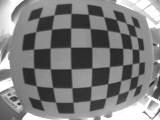
\includegraphics[width=\textwidth]{images/camera/0.png}
    \end{subfigure}
    \begin{subfigure}[b]{0.2\textwidth}
        \centering
        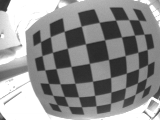
\includegraphics[width=\textwidth]{images/camera/1.png}
    \end{subfigure}
    \begin{subfigure}[b]{0.2\textwidth}
        \centering
        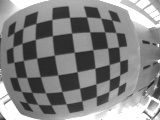
\includegraphics[width=\textwidth]{images/camera/2.png}
    \end{subfigure}
	\begin{subfigure}[b]{0.2\textwidth}
        \centering
        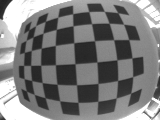
\includegraphics[width=\textwidth]{images/camera/3.png}
    \end{subfigure}
	\begin{subfigure}[b]{0.2\textwidth}
        \centering
        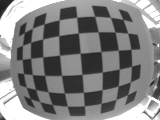
\includegraphics[width=\textwidth]{images/camera/4.png}
    \end{subfigure}
	\begin{subfigure}[b]{0.2\textwidth}
        \centering
        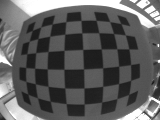
\includegraphics[width=\textwidth]{images/camera/5.png}
    \end{subfigure}
	\begin{subfigure}[b]{0.2\textwidth}
        \centering
        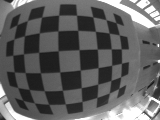
\includegraphics[width=\textwidth]{images/camera/6.png}
    \end{subfigure}
    \caption{\textbf{Training images used for camera model calibration} - The orientation and position of the chessboard were changed from one image to another to most of the field of view. The images are given in grayscale by the camera and exhibit a resolution of $160 \times 120$ pixels.}
    \label{fig:cameraImages}
\end{figure}

In the end, we obtained a subpixel average error of $0.34$ pixels and the following model, which relies on a 4\textsuperscript{th}-order Taylor polynomial:\\
\begin{center}
Polynomial:
$
\begin{cases}
a_0 = -6.66 . 10^{1}\\ 
a_1 = 0.00 \\
a_2 = 6.42 . 10^{-3} \\
a_3 = -2.31 . 10^{-5} \\
a_4 = 2.73 . 10^{-7} \\
\end{cases}
$
\hfill
Center:
$
\begin{cases}
x_c = 56.23 \\
y_c = 77.64 \\
\end{cases}
$
\hfill
Matrix:
$
\begin{cases}
c = 1.00 \\
d = -0.00 \\
e = -0.00 \\
\end{cases}
$
\end{center}
As we can see from the coefficients of the matrix in (\ref{equ:cameraModel2}), there is not significant misalignment between the camera and the lenses. Hence, we can neglect this part of the model if necessary. Nevertheless, the estimated location of the center is not exactly the actual center of the $160 \times 120$ grid of pixels. The reprojections of the points used for calibration appear on Figure~\ref{fig:cameraReproj}. 

This model was implemented as a structure which is passed as parameters to any function that needs it. The implementation of the projection from camera image to the (3D) scene is shown in Code~\ref{code:cameraModel}.
\newpage

\begin{figure}[h]
    \centering
    \begin{subfigure}[b]{0.4\textwidth}
        \centering
        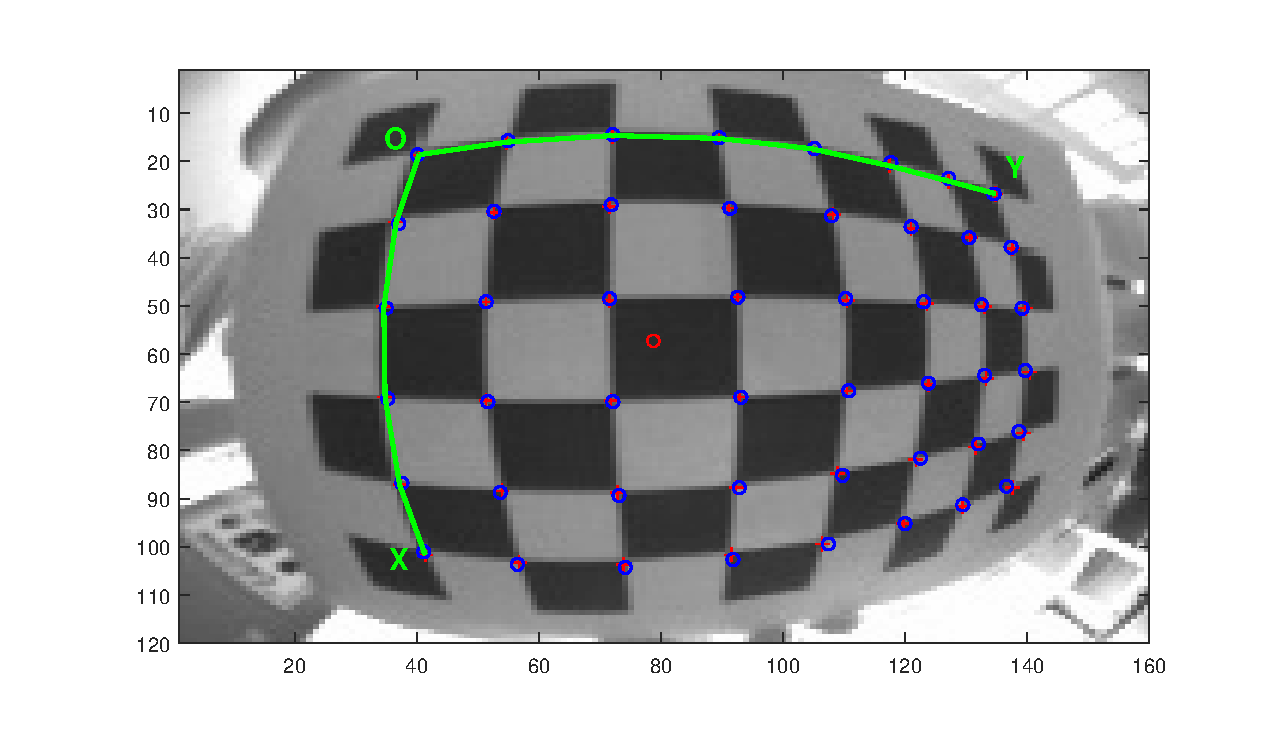
\includegraphics[width=\textwidth]{images/camera/Reproj7.eps}
    \end{subfigure}
    \begin{subfigure}[b]{0.4\textwidth}
        \centering
        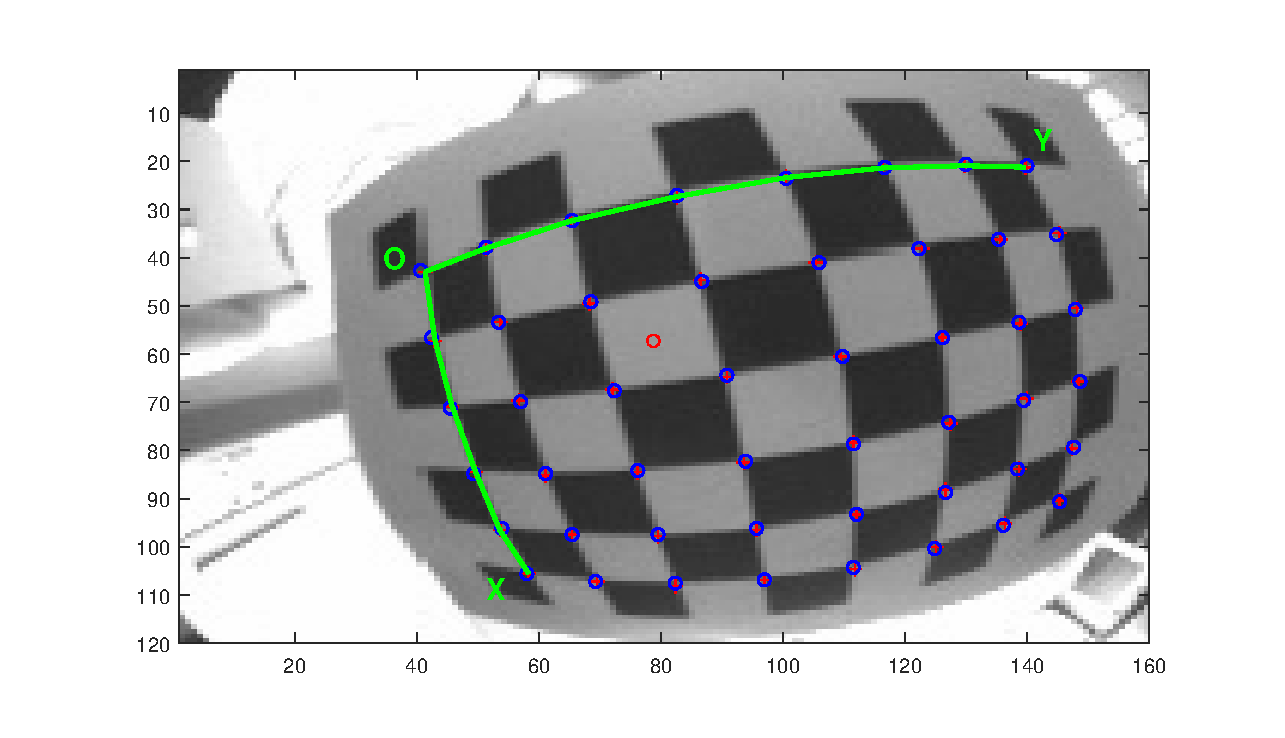
\includegraphics[width=\textwidth]{images/camera/Reproj6.eps}
    \end{subfigure}
    \begin{subfigure}[b]{0.4\textwidth}
        \centering
        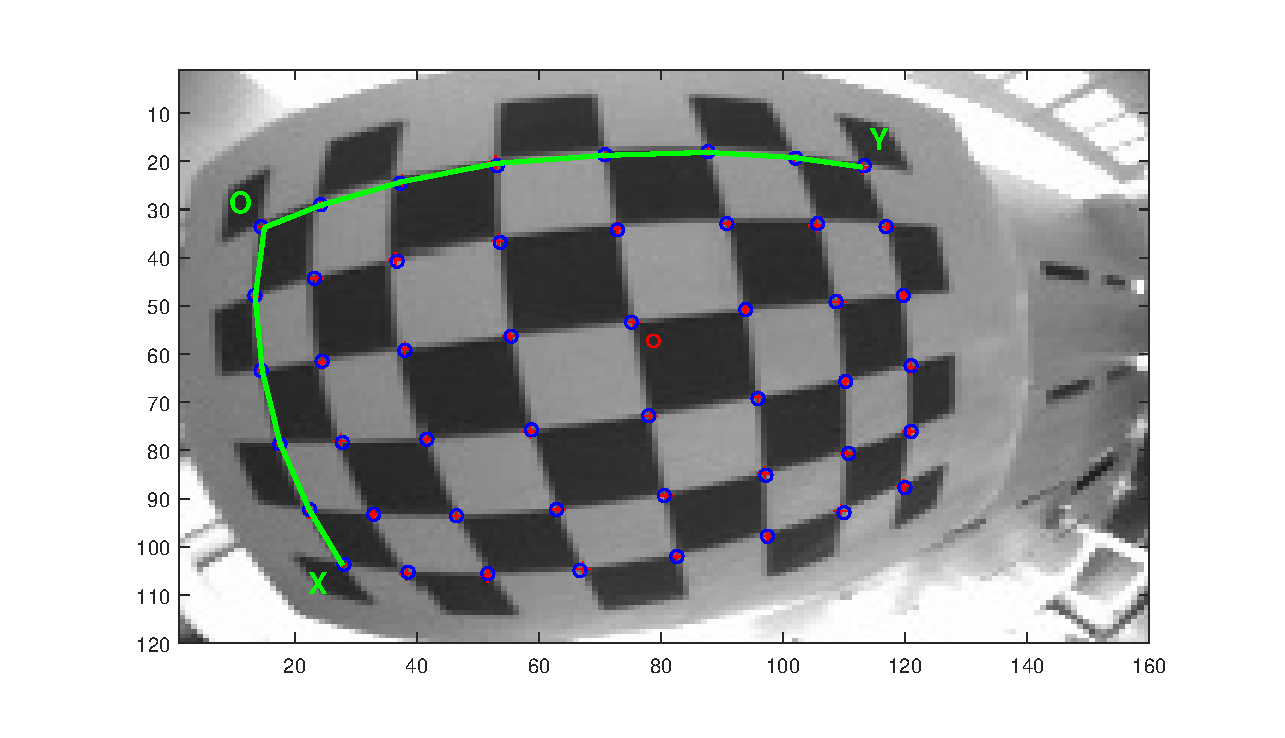
\includegraphics[width=\textwidth]{images/camera/Reproj5.eps}
    \end{subfigure}
	\begin{subfigure}[b]{0.4\textwidth}
        \centering
        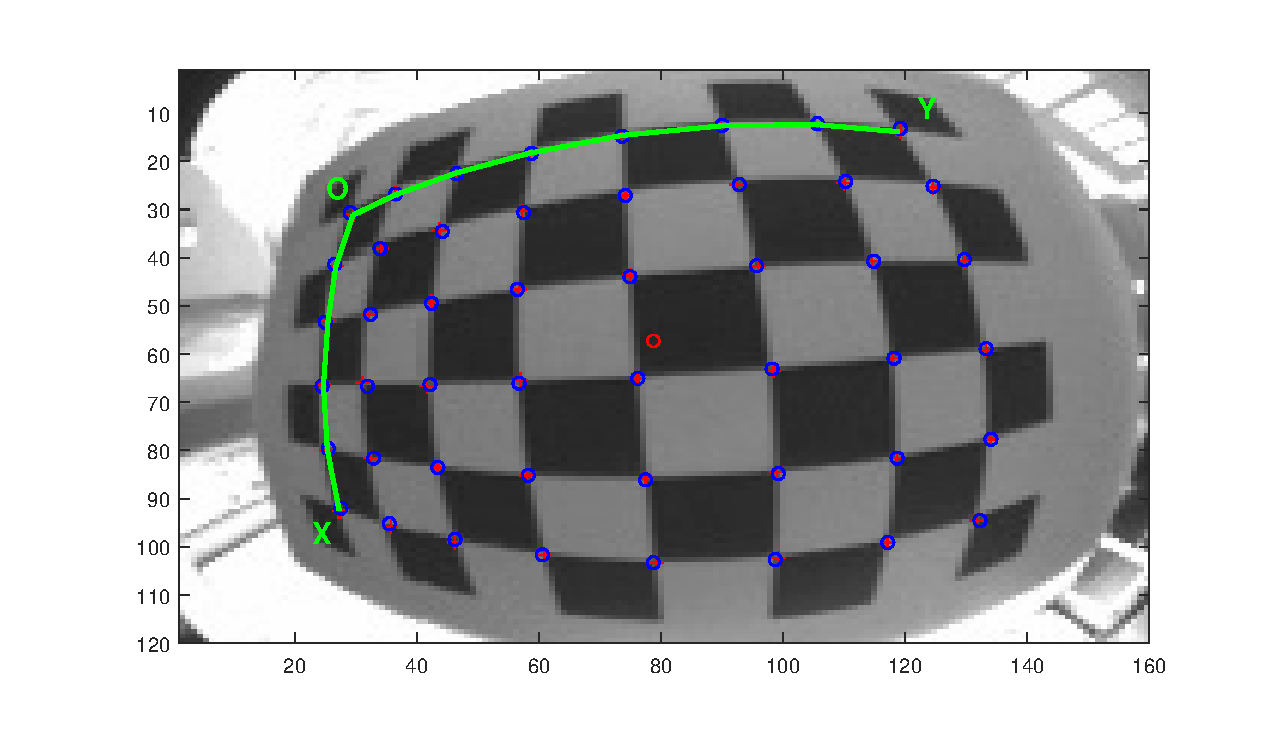
\includegraphics[width=\textwidth]{images/camera/Reproj4.eps}
    \end{subfigure}
	\begin{subfigure}[b]{0.4\textwidth}
        \centering
        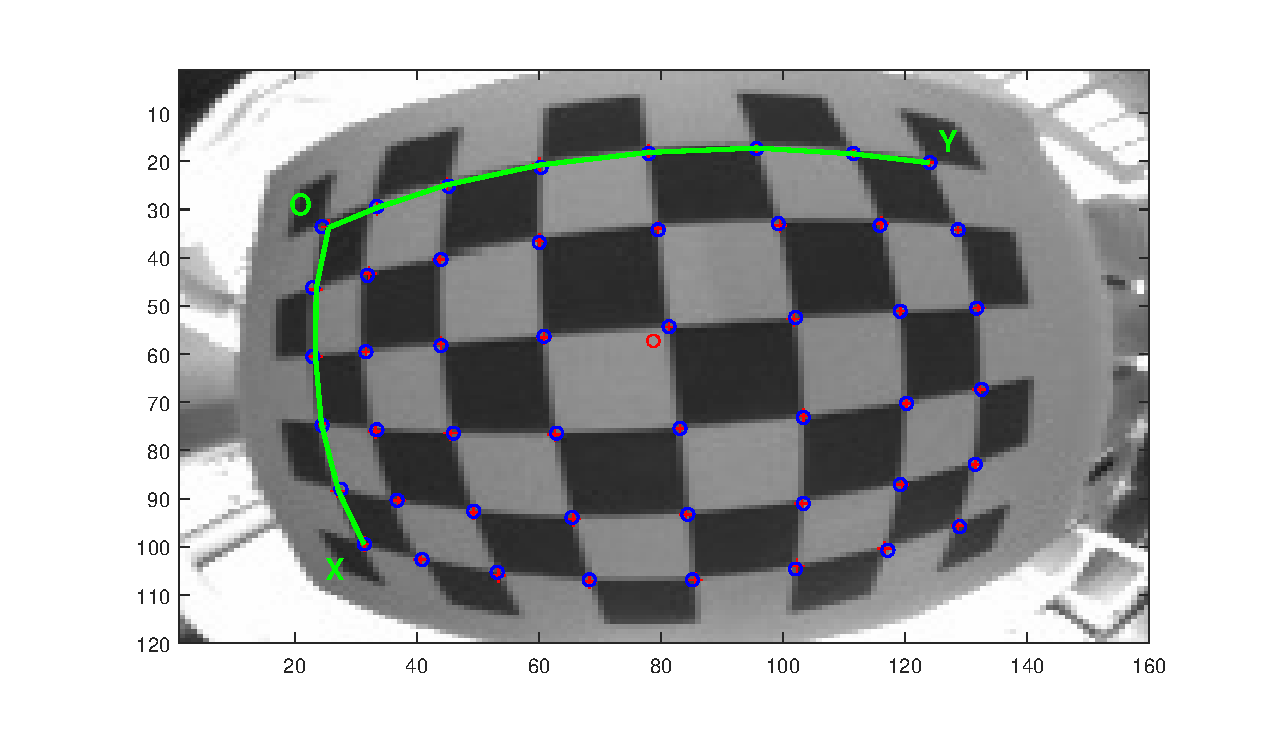
\includegraphics[width=\textwidth]{images/camera/Reproj3.eps}
    \end{subfigure}
	\begin{subfigure}[b]{0.4\textwidth}
        \centering
        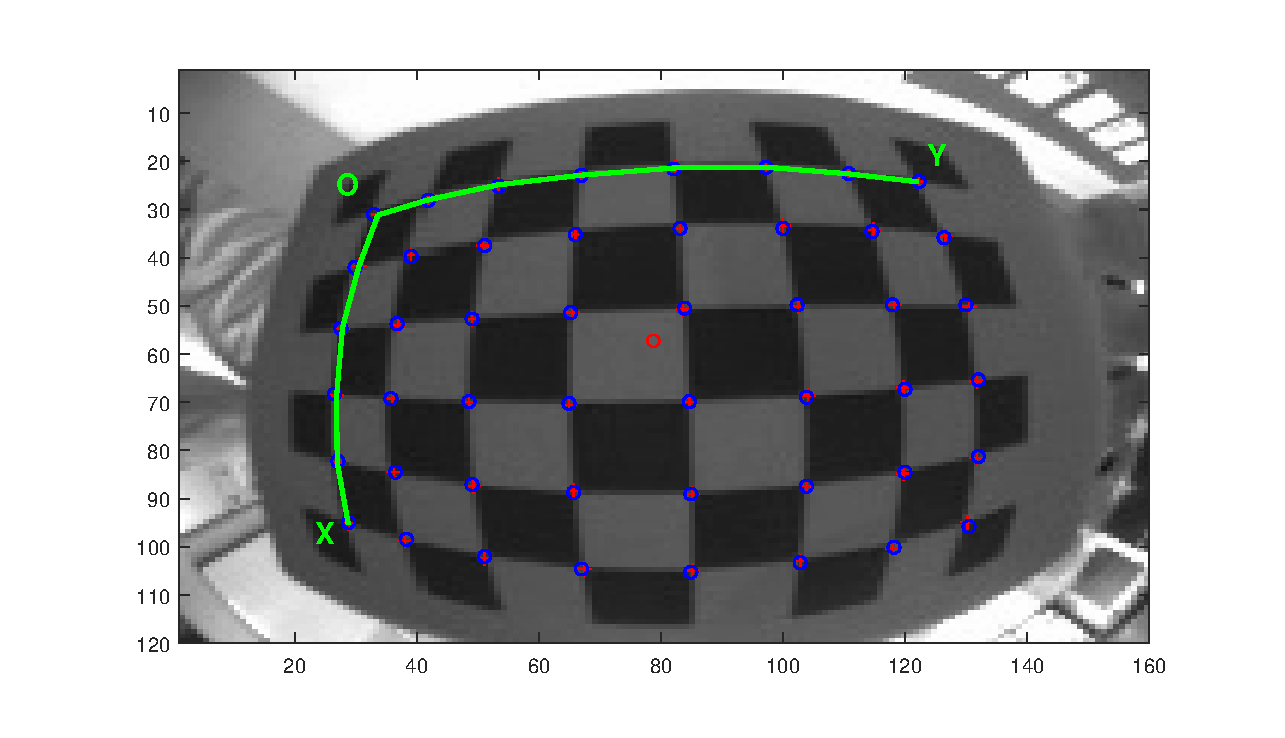
\includegraphics[width=\textwidth]{images/camera/Reproj2.eps}
    \end{subfigure}
	\begin{subfigure}[b]{0.4\textwidth}
        \centering
        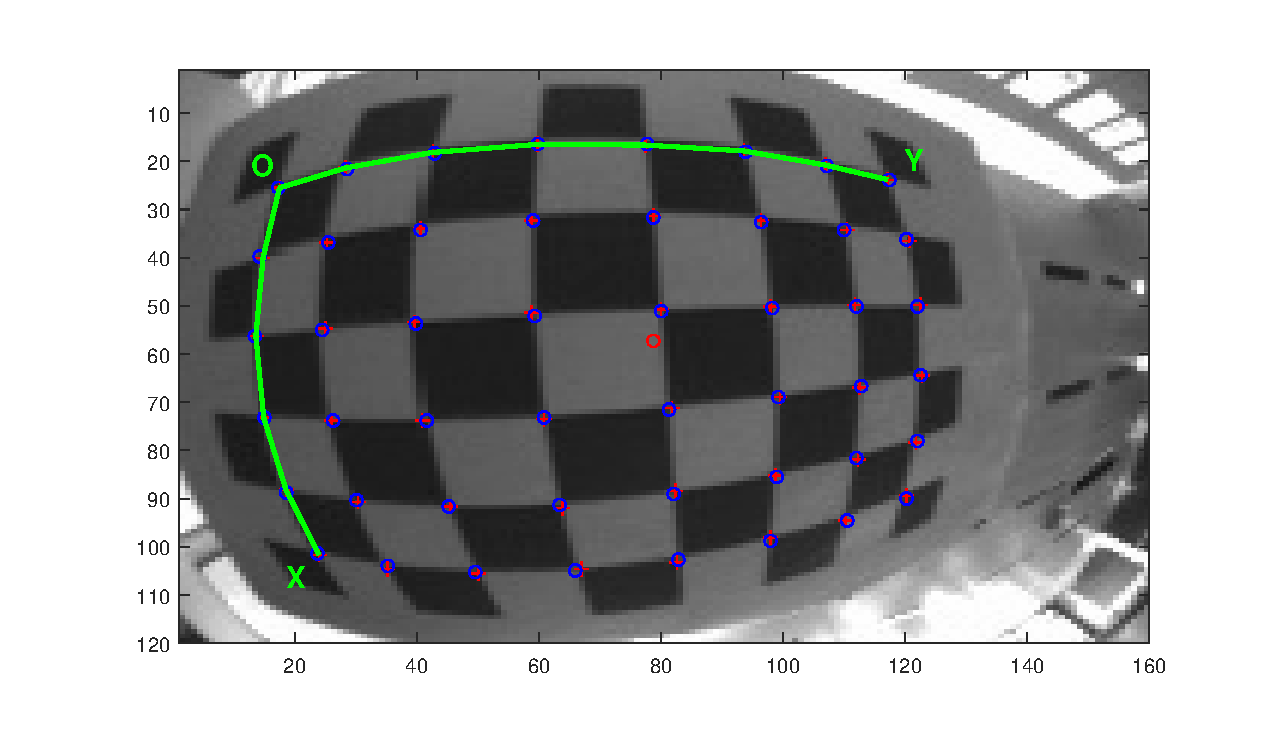
\includegraphics[width=\textwidth]{images/camera/Reproj1.eps}
    \end{subfigure}
    \caption{\textbf{Reprojection on the camera image after calibration}}
    \label{fig:cameraReproj}
\end{figure}
\newpage

\begin{center}
\begin{code}[colback=white, label=code:cameraModel]{From pixels to 3D directions}
void cam2world(float *xp, float *yp, float *zp, float u, 
		float v, cam_model *cam)
{
	 float *pol    = cam->pol;
	 float xc      = cam->xc;
	 float yc      = cam->yc; 
	 float c       = cam->c;
	 float d       = cam->d;
	 float e       = cam->e;
	 uint8_t length_pol = cam->length_pol;

	 float invdet  = 1/(c-d*e);

	 // back-projection of u and v
	 *xp = invdet*(    (u - xc) - d*(v - yc) );
	 *yp = invdet*( -e*(u - xc) + c*(v - yc) );
	  
	 float r = sqrt(SQR((*xp)) + SQR((*yp)));
	 *zp  	 = pol[0];
	 
	 float r_i = 1;
	 
	 // compute z from polynomial model
	 for (uint8_t i = 1; i < length_pol; i++)
	 {
	   r_i *= r;
	   *zp += r_i*pol[i];
	 }
}
\end{code}
\end{center}

\subsection{Mapping Optical Flow to Unit Sphere}
Now that the model of the omnidirectional camera is known - and the pixels can be mapped onto a plane or a sphere -, we can deduce the viewing direction corresponding to a given pixel. However, the particular geometry of the omnidirectional camera induces high distortions in the image. Hence, the optical flow, which is computed using Lucas-Kanade method, can be projected onto the unit sphere using the method presented in \cite{backproj}. Mapping the optical flow directly on the unit sphere allows us to simplify further processing required for the estimation of the location of the focus of expansion, through the straightforward use of spherical coordinates. However, though more natural, the sphere still induces radial distortions and may not be appropriate for all types of motions, as exposed by Shakernia et al.

The optical rays are described in spherical coordinates $(\rho, \theta, \Phi)$ from the center of the camera, where $\rho$ is the magnitude, $\theta$ is the azimuth in the $X$-$Y$ plane, and $\Phi$ is the polar angle between the ray and the $Z$-axis. Given an image point $(u,v)^T$, we first compute the corresponding ray (or back-projection ray) $b=(x, y, z)^T$ using equations (\ref{equ:cameraModel1}) and (\ref{equ:cameraModel2}), and normalize it to unit length $s = b/\|b\|$. The spherical coordinates of the "unitized" back-projection ray are given by:
\begin{equation}
\begin{cases}
\rho = 1\\[6pt]
\theta = \arctan(\dfrac{y}{x})\\[6pt]
\Phi = \arctan(\dfrac{r}{z})\\[6pt]
\end{cases}
\end{equation}
where $r = \sqrt{x^2+y^2}$. Using equations (\ref{equ:cameraModel1}) and (\ref{equ:cameraModel2}), we can derive the following Jacobian which relates the partial derivatives from the image plane to the unit sphere:
\begin{equation}
J =
\begin{bmatrix}
\dfrac{\partial\theta}{\partial u} & \dfrac{\partial\theta}{\partial v}\\[8pt]
\dfrac{\partial\Phi}{\partial u}	  & \dfrac{\partial\Phi}{\partial v}\\
\end{bmatrix}
=\dfrac{1}{det(A)}
\begin{bmatrix}
\dfrac{-y - ex}{r^2} & \dfrac{dy + cx}{r^2}\\[8pt]
\dfrac{d\Phi}{dr}\dfrac{(x-ey)}{r} & \dfrac{d\Phi}{dr}\dfrac{(cy - dc)}{r}\\
\end{bmatrix}
\end{equation}
where 
$
A = \begin{bmatrix}
c & d\\
e & 1\\
\end{bmatrix}
$
and 
$ \dfrac{d\Phi}{dr} = \dfrac{z - r\rho'(r)}{r^2 + z^2}$\\
Then, we compute the transformation which takes the partial derivatives on the unit sphere from spherical coordinates to rectangular coordinates:
\begin{equation}
S =
\begin{bmatrix}
-\sin\theta \sin\Phi & \cos\theta \cos\Phi\\
~~\cos\theta \sin\Phi & \sin\theta \cos\Phi\\
0 & -\sin\Phi\\
\end{bmatrix}
\end{equation}
Therefore, we can compute the mapping of an image point $(u,v)^T$ (considered distorted) and its corresponding optical flow $(\dot{u}, \dot{v})^T$ to the unit sphere:
\begin{align}
s &= b/\|b\| & \dot{s} &= SJ \begin{bmatrix} \dot{x} \\ \dot{y} \end{bmatrix}
\end{align}
A possible C implementation is detailed in Code~\ref{code:flowProjection}

\begin{center}
\begin{code}[colback=white, label=code:flowProjection]{Backprojection of optical flow}
void flow2world(float *flow_x, float *flow_y, float *flow_z, 
		float xp, float yp, float zp, float flow_u, 
		float flow_v, cam_model *cam)
{
	 float *pol    = cam->pol;
	 float c       = cam->c;
	 float d       = cam->d;
	 float e       = cam->e;
	 uint8_t length_pol = cam->length_pol;
	 float invdet  = 1/(c-d*e); 
	 
	 // from cartesian to spherical coordinates
	 float r   = sqrt(SQR(xp) + SQR(yp));
	 float theta = atan2(yp,xp);
	 float phi = atan2(r, zp); 
	 
	 // compute polynomial model derivative
	 float r_i = 1;
	 float dzp = pol[1];
	 for (uint8_t i=2; i < length_pol; i++)
	 {
	   r_i *=r;
	   dzp += i*pol[i]*r_i;
	 }
	 // project optic-flow on unit sphere
	 float d_thetau = invdet*(-yp/SQR(r) - e*xp/SQR(r));
	 float d_thetav = invdet*(d*yp/SQR(r) + c*xp/SQR(r));
	 float d_phir = (zp - r*dzp)/(SQR(zp) + SQR(r));
	 float d_phiu = d_phir*invdet*(xp/r - e*yp/r);
	 float d_phiv = d_phir*invdet*(-d*xp/r + c*yp/r);
	 float flow_theta = d_thetau*flow_u 
	 		   + d_thetav*flow_v;
	 float flow_phi = d_phiu*flow_u + d_phiv*flow_v;
	 
	 // from spherical to cartesian coordinates
	 *flow_x = -sin(theta)*qsin(phi)*flow_theta 
	 	   + cos(theta)*cos(phi)*flow_phi;
	 *flow_y = cos(theta)*sin(phi)*flow_theta 
	 	   + sin(theta)*cos(phi)*flow_phi;
	 *flow_z = -sin(phi)*flow_phi;
}
\end{code}
\end{center}

This method is obviously quite computationally expensive. Indeed, further testing on the camera board revealed that the computation of $117$ optic-flow vectors accounts for approximately 6ms. This value is to be compared to the refresh rate of our camera which is 200Hz. Thus, the runtime (for one iteration) is more than doubled by the use of the above method. 

In an attempt to reduce the computational overhead, we considered an approximate projection of the optic-flow measurement on the unit sphere. Considering the high refresh rate of the camera, any motion will induce a low displacement of the pixels on the camera image (i.e. a small optic-flow measurement). The latter remark allows us to take advantage of the small-angle approximation. More formally, we approximate the actual optic-flow projection $F$ to the difference between a sampling direction $P_1$ and a virtual point $P_2$ that is obtained from the projection of the point $p_2 = p_1 + f$, where $p_1$ is the point on the camera image corresponding to the 3D vector $P_1$ and $f$ is the 2D optic-flow:
\begin{align}
\begin{split}
{}&P_2 = g(p_2) = g(p_1 + f)\\
{}&F \approx P_2 - P_1\\
\end{split}
\end{align}
where $g$ is the spherical projection function described in the previous section and $F$ is the spherical projection of the optic-flow.

The resulting optic-flow vector is obviously not perpendicular to the sphere. However, building on the same assumption, we can neglect the radial component of the flow and simply use this raw vector for subsequent computations. The C implementation is shown in Code~\ref{code:fastFlowProjection}.

As for computational gain, running this version of the flow projection dramatically reduces the runtime with less than 2ms to process the $117$ optic-flow measurements.

\begin{center}
\begin{code}[colback=white, label=code:fastFlowProjection]{Fast backprojection of optical flow}
void fast_flow2world(float *flow_x, float *flow_y, 
		float *flow_z, float xp1, float yp1, 
		float zp1, float u1, float v1, 
		float flow_u, float flow_v, cam_model *cam)
{
	 // add optic-flow to pixel coordinates (u1, v1)
	 float u2 = u1 + flow_u;
	 float v2 = v1 + flow_v;

	 // define new coordinates
	 float xp2;
	 float yp2;
	 float zp2;

	 // map to 3d scene
	 cam2world(&xp2,  &yp2,  &zp2,  u2,  v2, cam);

	 // project on unit sphere
	 normalize(&xp2, &yp2, &zp2);

	 // compute optic-flow considering small angles
	 *flow_x = xp2 - xp1;
	 *flow_y = yp2 - yp1;
	 *flow_z = zp2 - zp1;
}
\end{code}
\end{center}

\subsection{Derotation of Optical Flow}
Under the assumption of differential motion, that is small translation and rotation of the camera between each frame, we can approximate the geometrical effects of egomotion on the perceived image motion to a first-order Taylor polynomial. Hence, as the scene is projected on the unit sphere centered on the vantage point, each optical flow measurement can be expressed as a 3D vector tangent to the unit sphere and perpendicular to the viewing direction:
\begin{equation}
\label{equ:opticflow}
f = -w \times d - \dfrac{v - (v \cdot d)d}{D}
\end{equation}
where $d$ is a unit vector describing the viewing direction, $w$ the angular speed vector, $v$ the translational velocity vector and $D$ the distance to the viewed object. The measured optical flow $f$ can be decoupled and expressed in two parts, namely the rotation-induced and the translation-induced optical flows, respectively $f_r$ and $f_t$.

As we are only interested in the estimation of the angle of attack (i.e. the direction of translation), only the translational part $f_t$ of the optical flow is required. Hence, we proceed to the removal of the rotational part $f_r$ of the optical flow through the process of derotation \cite{derotation}. If necessary, the main axis $Z$ of the camera can be automatically calibrated using the method proposed in \cite{autocalib}, so as to estimate the transformation from the gyroscope frame to the camera frame. Even after calibration, the derotation procedure may introduce additional noise to the optical flow measurement, all the more so that the rotational component is larger than the translational part of the optical flow. This may be exacerbated by the sensor bias compensation and noise reduction only achieved using averaging and low-pass filtering.

However, before proceeding to the derotation of the optical flow, we must first consider scaling the angular rate values. Indeed, once projected on the unit sphere, the optical flow is given in [frame\textsuperscript{-1}] whereas the gyroscopes measurements are [rad.s\textsuperscript{-1}]. Given the refresh rate of the camera, the conversion is straight forward: 
\begin{equation}
w\mathrm{[frame\textsuperscript{-1}]} = 0.005 \cdot w\mathrm{[rad/s\textsuperscript{-1}]}
\end{equation}

\subsection{Finding the Focus of Expansion}
In order to find the direction of translation, we use the derotated optical flow to constrain the translation direction to lie on a great circle. This great circle is the intersection of a plane - defined by the vector defined by the viewing direction $d$, its corresponding optical flow vector $p_t$ and the center of the sphere $O$ - with the unit sphere. Hence, each optic-flow vector gives us a constrain on the position of the focus of expansion (FOE), which can be located anywhere on the great circle. Although only two great circles are required to constrain the location of the FOE to two points (and thus to find the axis of motion), several measurements are used so as to recover from possible outliers and noise.

For a robust estimation of the direction of translation, two different approaches are possible. The first one relies on RANSAC (RANdom SAmple Consensus) and its variants. However, this first method implies several estimations of the location of the FOE based on randomly sampled measurements and may not be suitable for implementation on a microcontroller and fast refresh rate. Another approach is to find the best intersection of all the great circle arising from the optical flow measurements such as the Hough-reminiscent voting method proposed in \cite{lim}. Voting has the advantage of performing in constant time under increasing outlier proportions without any loss of accuracy. Its higher robustness and the fact that it does not require an optimization process make this method the most suitable for embedded robotics. 
 
% Let $\hat{p}_t = \dfrac{p_t}{\|p_t\|}$ be the normalized optical flow vector corresponding to the viewing direction $d$. A parametric equation of the great circle defined by these two normalized vectors is:
% \begin{equation}
% v(t)= cos(t)\cdot\hat{p}_t + sin(t)\cdot d
% \end{equation}
% From this equation, we can proceed to voting along the great circle corresponding to each optical flow measurement. For the procedure not to be too computationally heavy, we can perform a coarse voting to determine a first approximation for the location of the FOE. Then, we refine our estimate by projecting the great circle on a plane tangent to the unit sphere in the vicinity of the estimated location. Hence, the voting procedure is simplified by voting along lines in the plane and there are efficient algorithms to perform this task, such as the Bresenham line algorithm.

In order to simplify the mathematical representation of the great circles, we rely on their normal vectors. Indeed, since a great circle is the intersection of the sphere with a plane passing though its origin, it can be defined using one of the unit normal vectors.
Formally, for a unit vector $n = (n_x, n_y, n_z)^T$, a great circle on the unit sphere $S^2$ is defined as
\begin{equation}
C = S^2~\bigcup~\{ x|x^Tn = 0, x \in \mathbb{R}^3 \}
\end{equation}
This normal vector $n$ is readily computed using the cross-product,
\begin{equation}
n = \dfrac{d \times f_t}{\|d \times f_t\|}
\end{equation}
% Considering two great circles and their corresponding normal vectors, namely $n_i$ and $n_j$, we can compute their intersections $a_{ij}$ and $a_{ji}$,
% \begin{equation}
% \begin{cases}
% a_{ij} = n_i \times n_j\\
% a_{ji} = n_j \times n_i\\
% \end{cases}
% \end{equation}
% Hence, we can vote to the accumulator for either $a_{ij}$ and $a_{ji}$ for each pair of points. Of course, the intersection of the two great circles actually yields two points.
Thus, we can vote along a great circle, given its normal vector, by computing simple dot products (i.e. 3 multiplications and 2 additions).

In practice, the intersection of two great circles define 2 possible directions of translation. To disambiguate between the two, one may pick one of the two points and calculate the angle between it and the vector $f_t$. If the angle is larger than $\pi/2$ radians, then that point is the focus of expansion. Another possibility is to use an additional sensor (such as a sonar) to choose the correct direction. In order to improve the processing speed on the camera chip (and to avoid ambiguity), we only consider one hemisphere, that is half the number of possible directions of translation. In other words, we only determine the axis of translation rather than its direction and we work on the hemisphere defined by $z<0$.

The voting procedure requires the storage of evenly distributed vectors on the unit sphere. The minimal angle between these vectors define the resolution of the voting procedure. For tractability reasons, we cannot afford to vote on the complete unit sphere in one batch. Hence, we are considering an iterative method which can be divided in two phases. The first one is a coarse voting procedure where we compute a rough estimate of the direction of translation using a few directions sampled from one hemisphere. This estimate is then used in the next phase where we perform voting on a refined spherical grid of higher resolution but reduced spread. The complete voting procedure is detailed in Algorithm~\ref{algo:houghVoting}.

\begin{algorithm}[colback=white, label=algo:houghVoting]{Hough-reminiscent voting}
Select optic flow measurement $p_t$ and viewing direction $d$
Compute normal vector $n = \dfrac{d \times p_t}{\|d \times p_t\|}$
For i = 1 to $N_{coarse}$ do
   If $x_i^Tn = 0$ then
      Vote for direction $x_i$
   end if
end for
Find the bins with maximum votes. This gives the coarse estimate.
Rotate the refined bins to center them on coarse estimate
For j = 1 to $N_{refined}$ do
   If $x_j^Tn = 0$ then
      Vote for direction $x_j$
   end if
end for
Find the bins with maximum votes. This gives the fine estimate
\end{algorithm}

The refined voting requires rotating the refined bins, which we computed for the a predefined direction (in our case $z = (0,~ 0,-1)$). There are three ways to achieve this transformation, namely the rotation matrix, axis-angle and quaternion methods \cite{rotation}. From a computational point of view, the rotation matrix method is the cheapest one (6 additions and 9 multiplications) whereas the quaternion method is the most expensive (18 additions and 21 multiplications). However, it is easier for us to use the axis-angle representation and then convert it to a rotation matrix so as to perform the transformation on every bins. The latter convertion accounts for 13 additions and 15 multiplications but the subsequent processing will only require 6 additions and 9 multiplications, provided that we can store the entire rotation matrix. A C implementation is given in Code~\ref{algo:rotation}.

Obviously, this whole method is sensible to noise which could affect the voting procedure if the accumulator has a finite resolution. In our case, the coarse resolution was set to $31^\circ$ and the fine resolution was chosen as approximately $4^\circ$. The latter value is justified considering the resolution of the camera (which is around 1.5°/pixel) and the additional noise induced by derotation. The former value was chosen so as to limit the number of coarse bins. The voting bins were evenly distributed on the unit and generated using the icosahedron method. Table~\ref{tab:votingBins} summarizes the voting bins parameters.

\begin{table}[h!]
	\centering
	\begin{tabular}{|p{2cm}||p{3cm}|p{3cm}|p{3cm}|}
	   \hline
	   \multicolumn{4}{|c|}{Voting bins parameter} \\
	   \hline
	   Voting set & Region & Number of bins & Resolution ($^\circ$) \\
	   \hline
	   Coarse & Hemisphere & 25 & 31\\
	   \hline
	   Refined & Coarse estimate & 42 & 4\\
	   \hline
	\end{tabular}
	\caption{\textbf{Voting bins parameters}-The voting bins are evely distributed on the unit sphere and were generated using icosahedron method.}
	\label{tab:votingBins}
\end{table}

\begin{code}[colback=white, label=algo:rotation]{Hough-reminiscent voting}
void rotate_bins(voting_bins *bins, float best_x, 
						float best_y, float best_z, 
						float *r_dir_x, float *r_dir_y, 
						float *r_dir_z)
{
	if(best_x==0.0f, best_y==0.0f, best_z==-1.0f){
		for(uint8_t i=0; i<bins->size; i++){
			bins->x[i] = r_dir_x[i];
			bins->y[i] = r_dir_y[i];
			bins->z[i] = r_dir_z[i];
		} 
	}
	else{
		// store cosine and sine
		float c = -best_z;
		float s = maths_fast_sqrt(1 - SQR(c)); 

		//store axis
		float u_x = 1.0f*best_y;					
		float u_y = -1.0f * best_x;					
		float u_z = 0.0f;

		// compute rotation matrix
		float R[9];
		aa2mat(R, u_x, u_y, u_z, c, s);

		// compute rotated refined bins
		for(uint8_t i=0; i<bins->size; i++){
			bins->x[i] = r_dir_x[i]*R[0]+r_dir_y[i]*R[1]
							+r_dir_z[i]*R[2];
			bins->y[i] = r_dir_x[i]*R[3]+r_dir_y[i]*R[4]
							+r_dir_z[i]*R[5];
			bins->z[i] = r_dir_x[i]*R[6]+r_dir_y[i]*R[7]
							+r_dir_z[i]*R[8];
		} 
	}
}
\end{code}

\subsection{Computational cost}


\newpage
\clearpage
\section{Results \& Discussion}
This section is dedicated to the description of the results obtaine from several experiments based on the above algorithm. We first describe the performance of the algorithm simulated in Matlab using synthetic optic-flow measurements. Then, we consider comparing estimates given by the algorithm to the "ground truth" obtained form a high-precision motion capture system.

\subsection{Simulation on Matlab}
The algorithm described in the previous section was first implemented in C to work on the embedded hardware. However, in order to verify its efficiency the code was translated into Matlab as faithfully as possible to the code used on the optic-flow sensor. Thus, the inner-workings of the key functions (e.g. back-projection, voting, etc.) were kept the same and did not make use of equivalent Matlab built-in functions. 

The sampling pixels were chosen identical to the ones used on the vision system, i.e. 81 pixels were uniformly distributed on a rectangular grid of 160x120 (corresponding to the camera resolution). They are then back-projected onto the unit sphere using the method detailed above. The optic-flow measurements are generated using the first-order approximation (\ref{equ:opticflow}). Outliers are simulated by adding randomly generated tangent vectors to a subset of the optic-flow vectors. The resulting optic-flow vectors are derotated and the normal vectors corresponding to the great circles are computed in the same way as in the C implementatin. Finally, voting is performed and the best estimate is found and compared to the actual direction of motion set by the user.

We first consider a single refinement stage in the estimation of the direction of translation. Then, 3 more stages are added as stated in the previous section. The parameters that were used are detailed in Table~\ref{tab:simParam}.
\begin{table}[h]
\centering
\begin{tabular}{|c|c|c|c|}
\hline
Velocity ($V$) & Angular rate ($w$) & Depth of scene ($D$) & Samples ($P$)\\
\hline
$[0.56, 0.42, 0.13]$ & $[0, \pi/3, \pi/5]$ & $50\cdot10^{-2}$ & 81\\
\hline
\end{tabular}
\caption{\textbf{Simulation parameters} - The velocity and angular rates were divided by the frequency of the camera (200Hz) to emulate real optic-flow computation\label{tab:simParam}}
\end{table}
Figures~\ref{fig:simOpticFlow}-\ref{fig:simDerotation} depicts respectively the sampling points and the optic-flow vectors, the outliers and the final set of vectors after derotation.

\begin{figure}
\centering
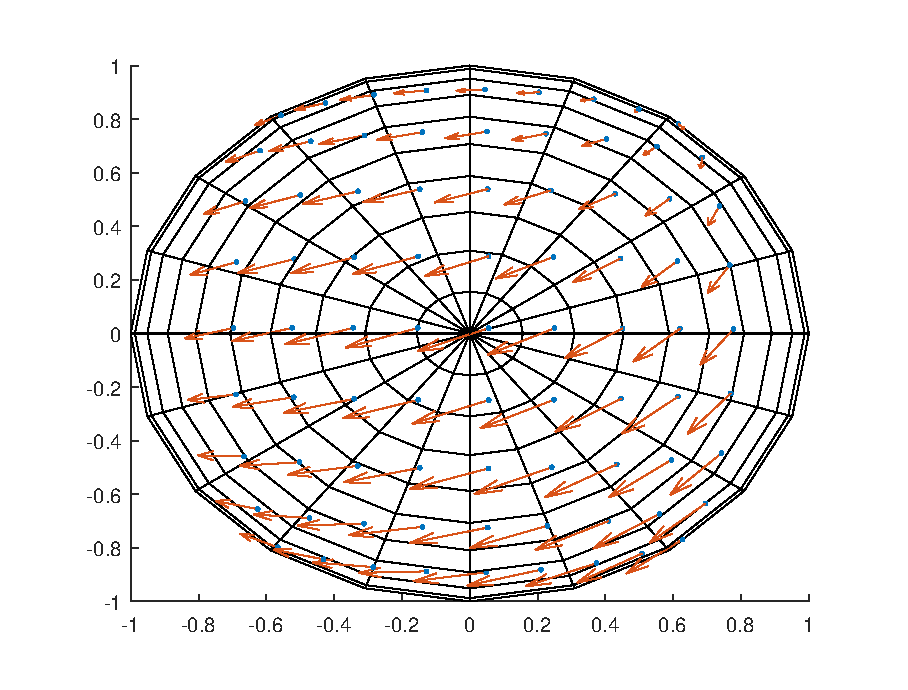
\includegraphics[width=0.6\linewidth]{images/matlab/simOpticFlow.eps}
\caption{\textbf{Generated sampling points and optic-flow vectors} - Synthesized using the first-order approximation and the parameters detailed in Table~\ref{tab:simParam}}
\label{fig:simOpticFlow}
\end{figure}

\begin{figure}
\centering
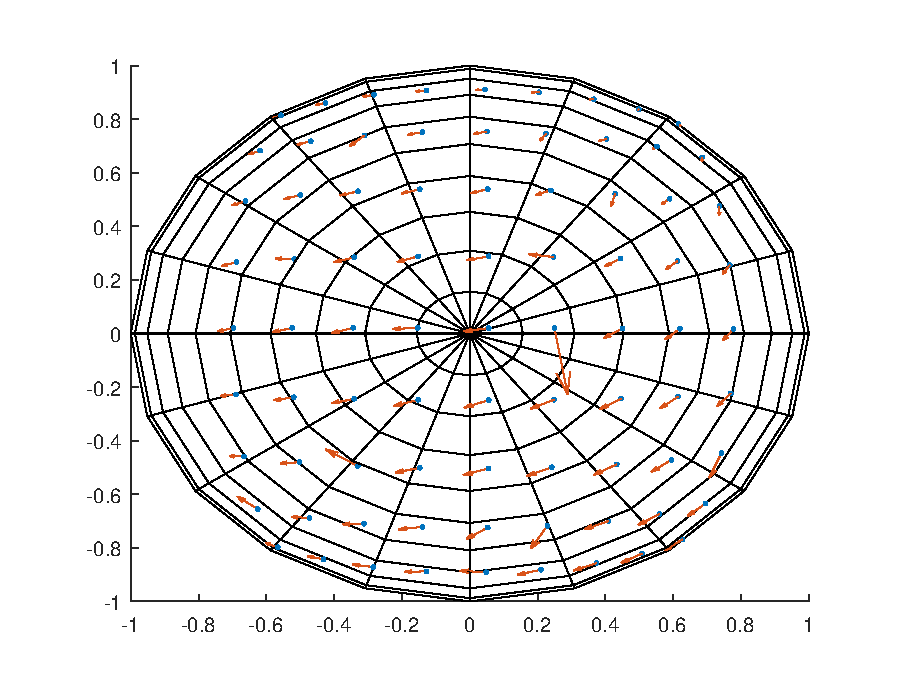
\includegraphics[width=0.6\linewidth]{images/matlab/simOutliers.eps}
\caption{\textbf{Generated outliers} - Synthesized using the first-order approximation and the parameters detailed in Table~\ref{tab:simParam} and additional randomly generated tangent vectors}
\label{fig:simOutliers}
\end{figure}

\begin{figure}
\centering
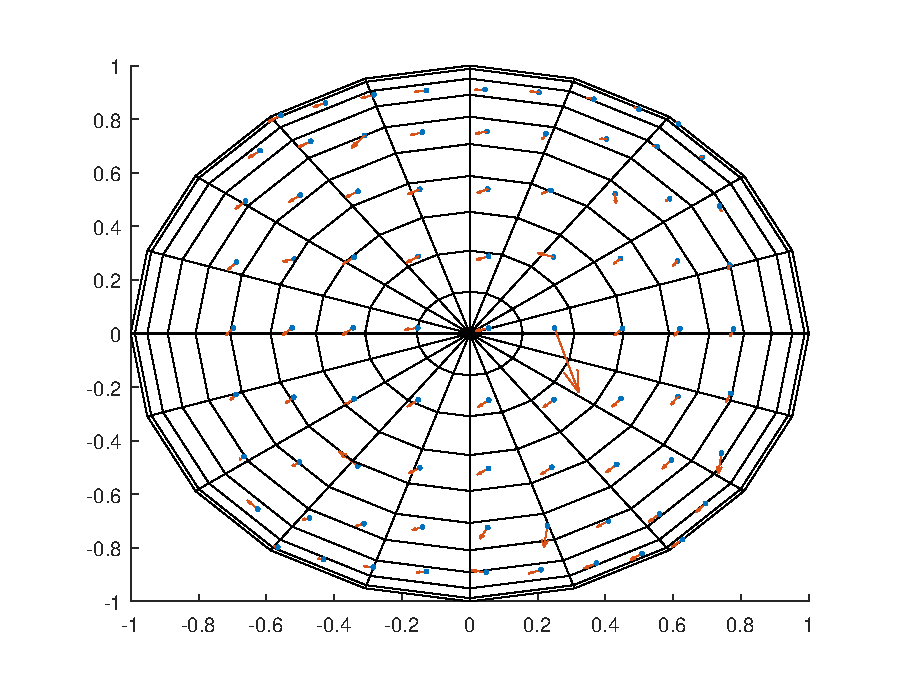
\includegraphics[width=0.6\linewidth]{images/matlab/simDerotation.eps}
\caption{\textbf{Derotated optic-flow vectors} - Synthesized using the first-order approximation and the parameters detailed in Table~\ref{tab:simParam} and additional randomly generated tangent vectors}
\label{fig:simDerotation}
\end{figure}

Both versions of the algorithm (Table~\ref{tab:votingBins}) are applied on synthetic optic-flow field with varying proportions of outliers. These outliers are randomly generated using the same seed for a fair comparision between the two. The results are averaged over 100 runs and correspond to the values of the dot products between the estimated and real directions of motion (which are unit vectors). 

From Table~\ref{tab:simResults}, it can be inferred that using fewer voting stages makes the algorithm slightly less sensible to outliers (at the expense of a significantly higher computational cost). Indeed, more stages means that outliers may still be present in intermediary stages and influence the estimate, all the more so when their proportion is greater than the one of the inliers. As the latter case may be rare in reality or avoided through the use of a quality factor on the optic-flow measurements, one may consider finding a trade-off between the number of stages (i.e. lowering the runtime) and the number of bins in each stage (i.e. the robustness and accuracy).

\begin{table}
\centering
\begin{tabular}{|c|c|c|c|c|}
\hline
\multirow{2}{*}{Stages} & \multirow{2}{*}{Accuracy} & \multicolumn{3}{c|}{Proportion of outliers}\\
\cline{3-5}
  & & 25\% & 50\% & 75\% \\
\hline
\multirow{2}{*}{2}  & Mean & 0.999782 & 0.999782 & 0.850839 \\
\cline{2-5}
& Std. dev. & 0.000000 & 0.000000 & 0.320995 \\
\hline
\multirow{2}{*}{5}  & Mean & 0.999913 & -0.999180 & 0.849634 \\
\cline{2-5}
& Std. dev. & 0.000000 & 0.002944 & 0.322923 \\
\hline
\end{tabular}
\caption{\textbf{Influence of outliers on estiamte} - The dot products of the estimated and real directions of motion are averaged over 100 runs with various proportions of outliers\label{tab:simResults}}
\end{table}


\subsection{Experiments with motion capture}
\subsubsection{Setup}
Experiments were conducted moving the camera by hand in a synthetic environment (i.e. textured walls) while recording its full displacement thanks to a motion capture system. These experiments were meant to assess the performance of the method described in Section II for estimating the direction of motion but may not be representative of its actual robustness under all conditions (different illumination, environment textures, etc.).

The optic-flow sensor consists in a PX4Flow board which integrates a 168MHz Cortex M4F CPU, a 3-axis rate gyro, a sonar, and the actual machine vision sensor. The biases and noise of the gyro are compensated by averaging and low-pass filtering and the scaling factor for derotation is stored in memory. A Sunex DSL215 fisheye lens is mounted on the board, allowing for a 185 degrees diagonal field of view in full frame format. The camera image is 160x120 pixel wide and sampled at 200Hz. All computations are performed on the chip and the estimates of the direction of motion are sent via USB and logged through QGroundControl (v.2.7).

We sample up to 117 optic-flow at each iteration ($\sim$160Hz), the latter of which are estimated using the Lucas-Kanade method on 10x10 binned image (patch). The vantage points corresponding to the optic-flow measurements are evenly distributed on the (rectangular) camera image. Although evenly-distributing points on the unit sphere was first considered - as it allows to uniformly sample the field of view -, this latter solution would imply overlapping in the binned image, thus increasing the statistical probability of encountering outliers. To cope with this issue, one may choose to adapt the size of the neighborhood (image patches) used in the optic-flow computation as proposed in \cite{adapted_neighborhood}.

% Describe optic-flow sensor board (chip + gyroscope)
% Describe lens (sunex)
% Describe sampling directions and number (and why)
% Describe image caching (built in function) and gyroscope sampling (same)
% Describe the remaining elements (sampling rate, algorithm run on chip)

% Descripton: PX4Flow is an optical flow smart camera (it provides the image for setup purposes, but it not designed to capture images like a webcam). It has a native resolution of 752�480 pixels and calculates optical flow on a 4x binned and cropped area at 400 Hz, giving it a very high light sensitivity. Unlike many mouse sensors, it also works indoors and in low outdoor light conditions without the need for an illumination LED. It can be freely reprogrammed to do any other basic, efficient low-level computer vision task.

% 168 MHz Cortex M4F CPU (128 + 64 KB RAM)
% 752�480 MT9V034 image sensor, L3GD20 3D Gyro
% 16 mm M12 lens (IR block filter)
% Size 45.5 mm x 35mm
% Power consumption 115mA / 5V

% \begin{itemize}
% \item MT9V034 machine vision CMOS sensor with global shutter
% \item Optical flow processing at 4�4 binned image at 400 Hz
% \item Superior light sensitivity with 24�24 �m super-pixels
% \item Onboard 16bit gyroscope up to 2000�/s and 780 Hz update rate, default high precision-mode at 500�/s
% \item Onboard sonar input and mount for Maxbotix sonar sensors. (HRLV-EZ4 recommended, SparkFun Product Link)
% \item USB bootloader
% \item USB serial up to 921600 baud (including live camera view with QGroundControl)
% \item USB power option
% \end{itemize}

% High Resolution Fisheye Lens:

% The DSL215 lens is a multi-megapixel miniature fisheye lens that achieves a 185 degree diagonal field of view on 1/4" format (full frame):
% Specifications:

% \begin{itemize}
% 	\item Imager format: 1/4"
% 	\item Focal length: 1.55mm (enables good low light performance)
% 	\item Relative aperture: F/2.0
% 	\item Image circle: 4.7mm
% 	\item Field of view: 138� at 3.6mm image circle / 185� at 4.7mm image circle
% \end{itemize}

% The optic-flow measurements are sampled at 200Hz while the full direction of motion estimation algorithm is run on the optic-flow sensor chip. 
\begin{figure}[h]
\centering
\includegraphics[width = 0.5\linewidth]{images/moCapFrame.jpg}
\caption{\textbf{Optic-flow sensor mounted on its motion capture frame} - The frame is equipped with 5 passive markers attached at known positions to obtain 3D position and orientation of the rigid body out of the 21 IR cameras.}
\label{fig:motionCapture}
\end{figure}

Experiments were performed using an OptiTrack motion capture system which high precision allowed to estimate the ground truth measurements. The optic-flow sensor was mounted on a frame equipped with 5 markers (coated with a reflective material) attached at known positions to obtain the three-dimensional position and orientation of the rigid body (Fig.~\ref{fig:motionCapture}). The motion of the camera was recorded at 250Hz using a set of 21 IR cameras. The measured orientation are differentiated so as to obtain the angular rates of the rigid body, which are compared to the gyroscopes measurements for synchronization purposes (convolution).


Motion capture using passive markers requires the emission of IR lights that are sensed by the camera due to its small size. Due to the frequency at which these articial lights were emitted (250Hz), the ambiant illumination as seen by the camera (200Hz) typically changed every 150ms inducing an automatic calibration of the luminosity, which requires extra 5ms before new readings are sampled. Although this setup was kept due to time constraints, this issue could be avoided by switching of IR lights and using active markers (i.e. a set IR LEDs).

\subsubsection{Results}
The experiments were performed using the algorithm detailed above with 5 stages refinements. The number of samples was first fixed to 81, which typically enables a runtime of 5.3ms ($\sim$ 180Hz); and then slightly increased up to 117 samples. As the results are mostly similar in both cases, we will focus on the lower number of samples in the remaining of this part.

As the measurements obtained from the optic-flow sensor and the motion capture system were not started simultaneously, we had to synchronize them afterwards. To ease up the process, we performed a recognizable motion that involved the gyroscope of the camera. Indeed, the gyroscope measurements are typically much less noisy than the optic-flow data. Hence, the angular rates measured by the optic-flow sensor were stored and compared to the estimates of the rates inferred from the motion capture system. The derivatives of the quaternions given by OptiTrack were computed using the three points rule, which typically allows for a better estimate. They were then converted from global to local (camera) coordinates. The synchronization was realized manually as recognizable features were easily located. Note that since the two systems exhibit different refresh rates, the values of the camera gyroscope were interpolated using a standard linear regressor between each datapoint. Finally, one may consider smoothing the data (e.g. using a gaussian window) though this was not required for synchronizing the signals in our case. Some results of the synchronization process are shown in Figures~\ref{fig:mocapGyro81X}-\ref{fig:mocapGyro81YZ}.

\begin{figure}
\centering
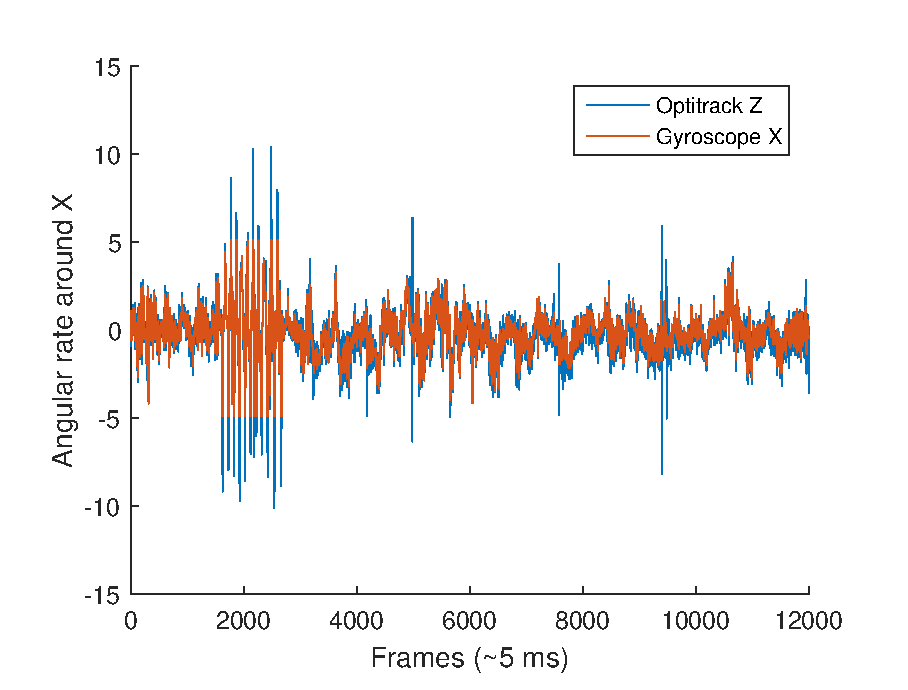
\includegraphics[width = 0.8\linewidth]{images/matlab/mocapGyroX81}
\caption{\textbf{Synchronized signals from camera and OptiTrack (X axis)} - The signals were synchronized manually using recognizable features (e.g. around frame 2000). The axes of the optitrack were circularly permutated so as to correspond to the ones of the camera frame.}
\label{fig:mocapGyro81X}
\end{figure}

\begin{figure}
\centering
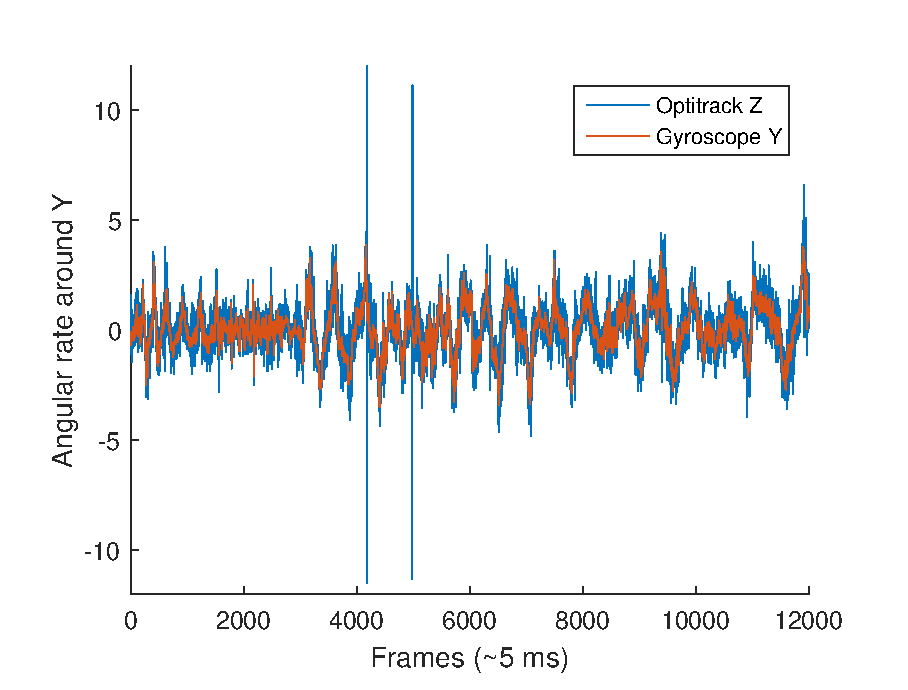
\includegraphics[width = 0.48\linewidth]{images/matlab/mocapGyroY81}
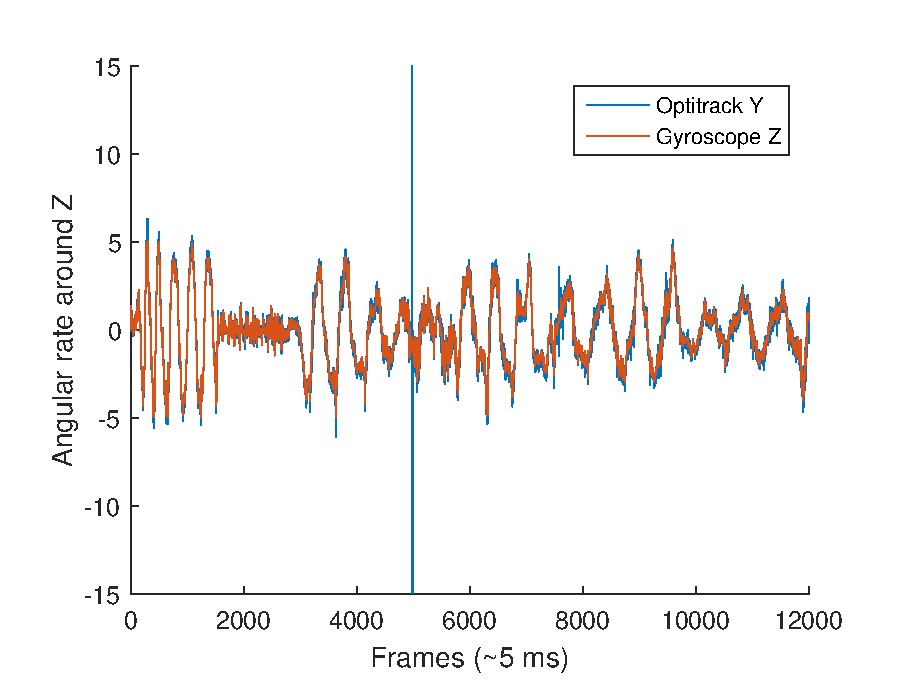
\includegraphics[width = 0.48\linewidth]{images/matlab/mocapGyroZ81}
\caption{\textbf{Synchronized signals from camera and OptiTrack (Y \& Z axes)} - The signals were synchronized manually using recognizable features. The axes of the optitrack were circularly permutated so as to correspond to the ones of the camera frame.}
\label{fig:mocapGyro81YZ}
\end{figure}

As it can be seen on Figures~\ref{fig:mocapGyro81X}-\ref{fig:mocapGyro81YZ}, both signals display comparable accuracy although some spikes are visible on the OptiTrack estimates. These spikes may be due to markers being lost by the motion capture system (thus inducing very fast changes in the orientation of the rigid body).

The direction of motion was estimated from motion capture outputs using the 3 points rule on the 3D position. This so-called "ground-truth" is compared to the optic-flow sensor estimates by considering the absolute value of the estimates (as only the axis of motion is estimated by the optic-flow sensor). To cope with the high oscillations observed in both signals, the raw measurements obtained for 81 viewing directions were smoothed using gaussian windows. The first one, which is equivalent to a $\sigma=20ms$, yields the graph shown in Figure~\ref{fig:mocapPos81_sig20}. Both signals seem to follow the same trend although the optic-flow sensor estimate still exhibit high error when compared to the motion capture measurements. By increasing the width of the gaussian window ($\sigma = 100ms$), the estimates still appear correlated, meaning that our method is correct but our estimates remain poor (Fig.~\ref{fig:mocapPos81_sig100}). 

\begin{figure}
\centering
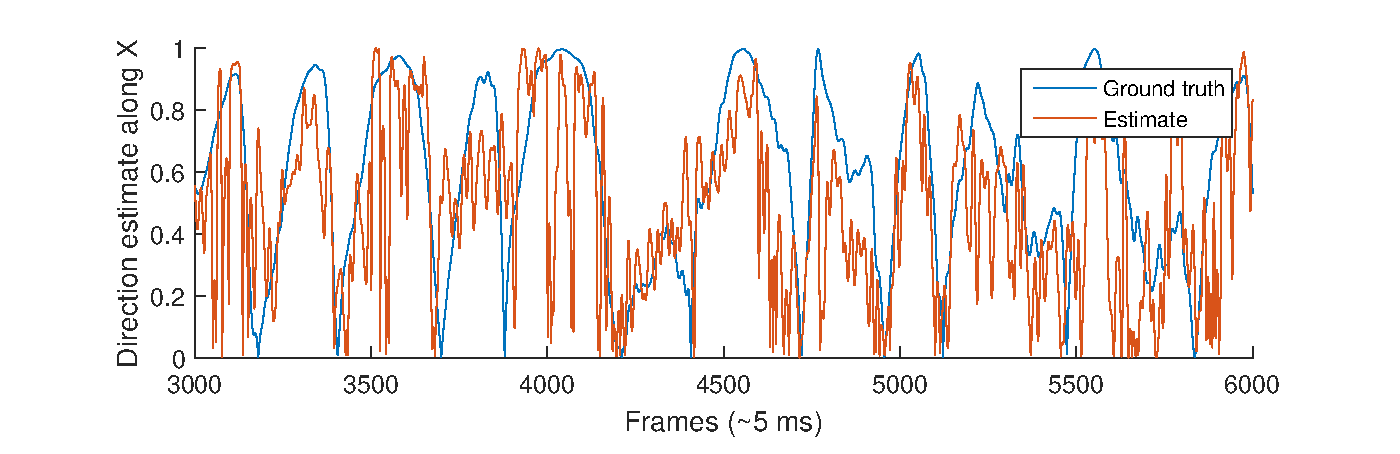
\includegraphics[width = \linewidth]{images/matlab/comparison_sig_20_X}
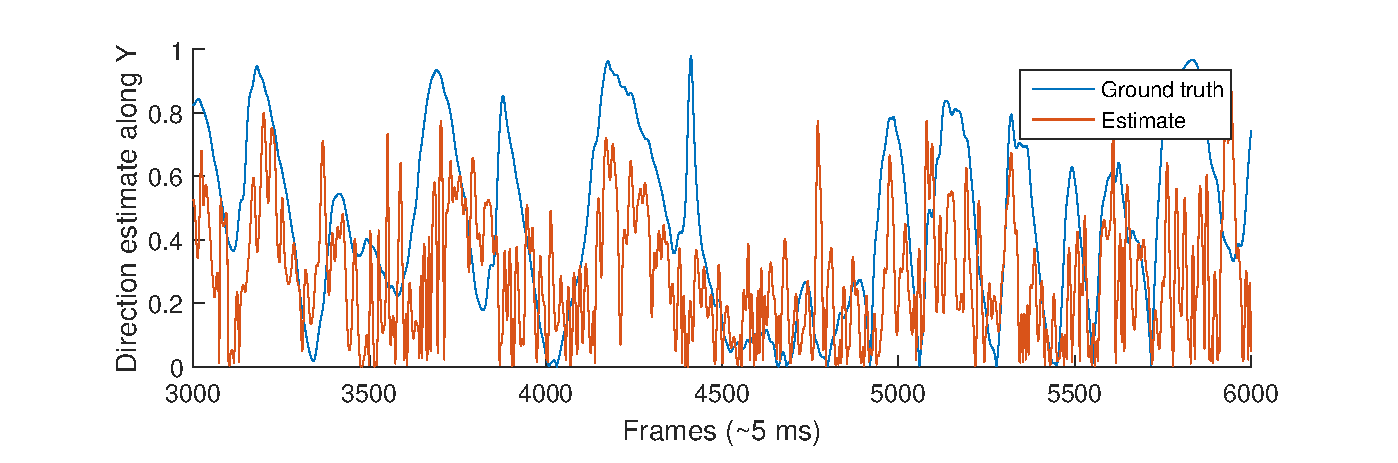
\includegraphics[width = \linewidth]{images/matlab/comparison_sig_20_Y}
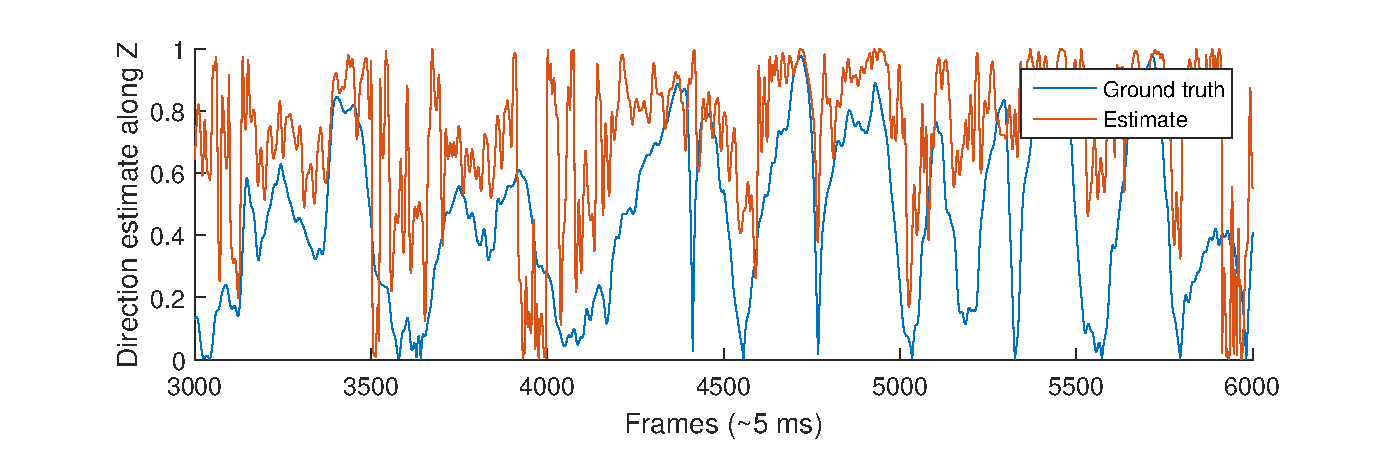
\includegraphics[width = \linewidth]{images/matlab/comparison_sig_20_Z}
\caption{\textbf{Comparison of optic-flow sensor estimates with "ground-truth" (20 ms gaussian window)} - The signals appear to follow the same trend although the optic-flow estimates are still very noisy. \label{fig:mocapPos81_sig20}}
\end{figure}

\begin{figure}[t]
\centering
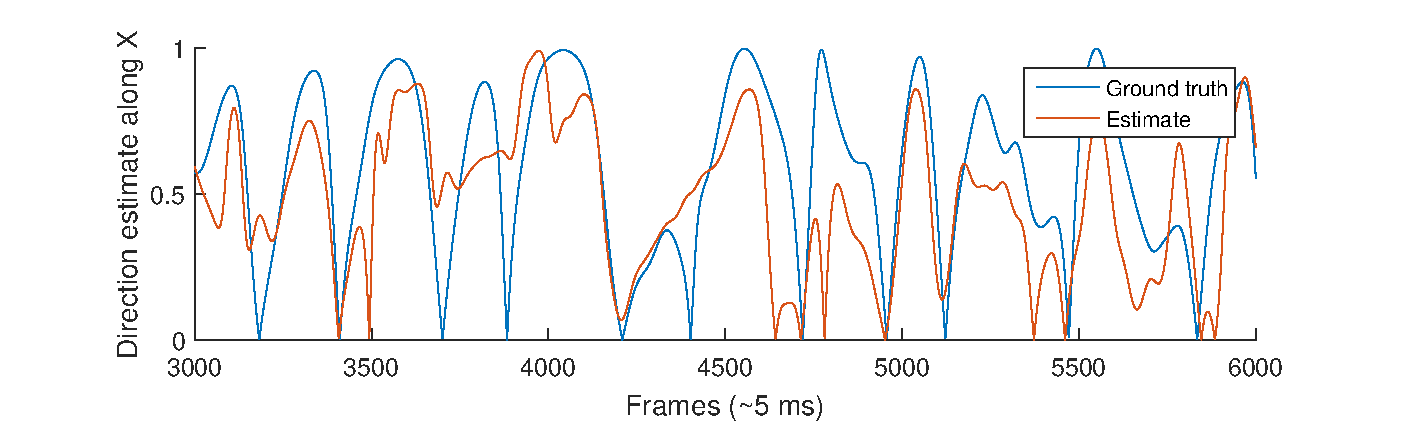
\includegraphics[width = \linewidth]{images/matlab/comparison_sig_100_X}
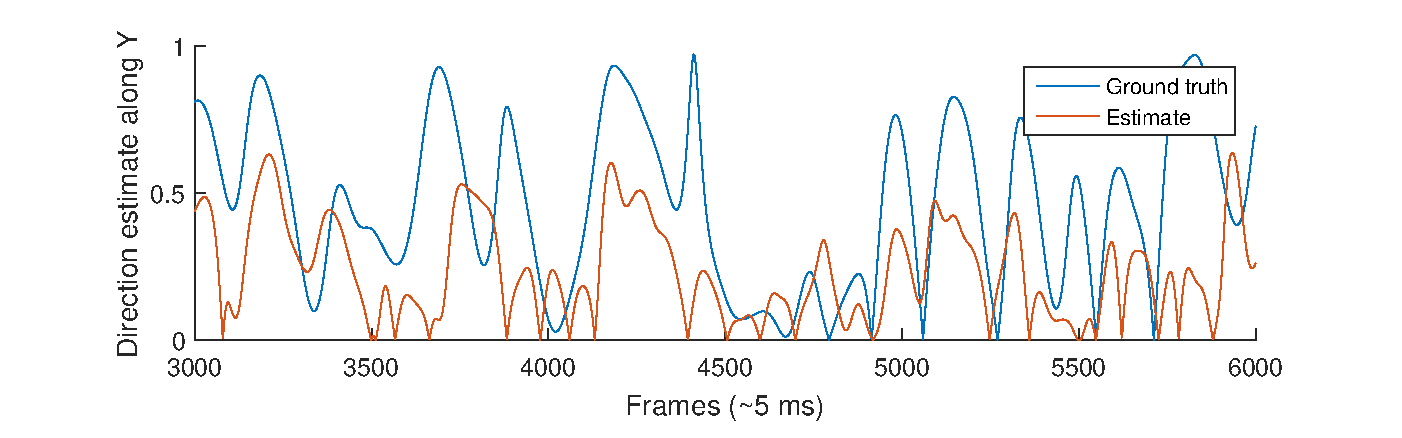
\includegraphics[width = \linewidth]{images/matlab/comparison_sig_100_Y}
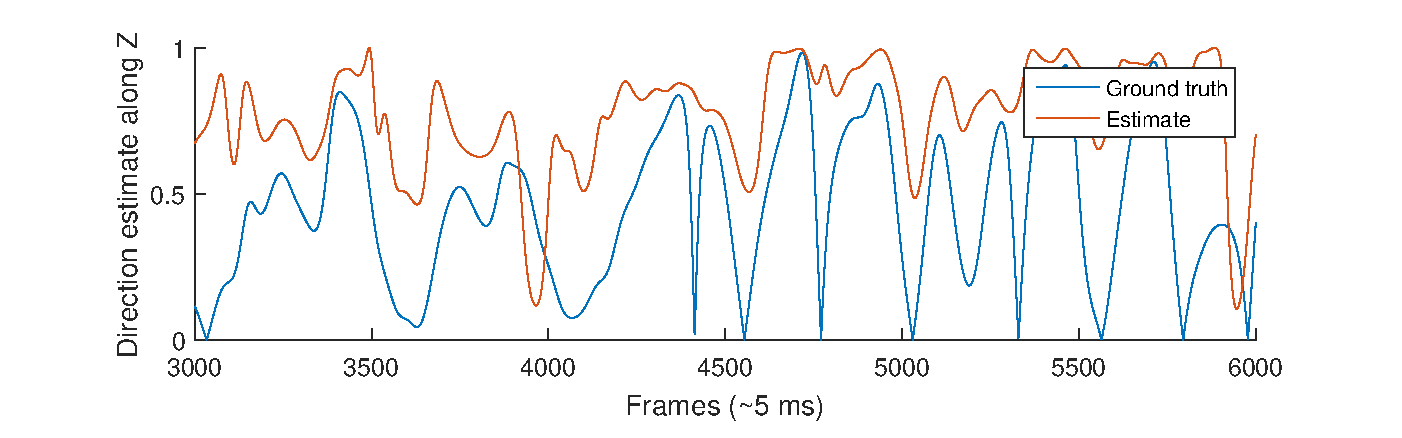
\includegraphics[width = \linewidth]{images/matlab/comparison_sig_100_Z}
\caption{\textbf{Comparison of optic-flow sensor estimates with "ground-truth" (100 ms gaussian window)} - The signals appear to follow the same trend although the optic-flow estimates still exhibit a high error. \label{fig:mocapPos81_sig100}}
\end{figure}

The accuracy of the estimation is computed using the absolute value of the dot product of the (normalized) estimated direction and the (normalized) ground truth at each frame. The results are summarized in Table~\ref{tab:mocapStatistics}. As can be seen, the method exhibit a very low average accuracy, which is slightly higher than $50^o$. Surprisingly enough, the overall accuracy is even way lower than the simulated one in the worst conditions (i.e. with 75\% outliers).

As the latter statistics are not fully representative of the actual performance, the accuracy at each time step was plotted in Figure~\ref{fig:mocapAccuracy81}. The system displays regular drops in the accuracy of his estimate. This drops may be related to rapid changes in the motion of the camera, the latter of which were quite frequent when moving the camera by hand.

\begin{table}
\centering
\begin{tabular}{|c|c|c|}
\hline
\multirow{2}{*}{Statistics} & \multicolumn{2}{|c|}{Width of the Gaussian window}\\
\cline{2-3}
& $\sigma = 20ms$ & $\sigma = 100ms$\\
\hline
Mean & 0.692394 & 0.669445 \\
\hline
Std. dev. & 0.274798 & 0.277248 \\ 
\hline
Max & 0.999980 & 0.999988 \\
\hline
Min & 0.000097 & 0.000054 \\
\hline
\end{tabular}
\caption{\textbf{Statistics from the motion capture experiments} - The accuracy corresponds to the absolute value of the dot product between both (normalized) direction of motion estimates (optic-flow sensor and motion capture system). The optic-flow sensor yields really poor average accuracy which is slightly higher than $50^o$.\label{tab:mocapStatistics}}
\end{table}

Nevertheless, in all cases, the values are far from the "ground truth", even when more samples are processed. Unfortunately, whether or not the changing ambiant lighting has influenced the estimation of the direction of motion remains an open question. Finally, considering the quality of the data gathered from optic-flow processing, it may be sensible to perform further post-processing on the estimates, such filtering or averaging, which will most likely improve performance at the expense of a lower sensitivity (or slower response time) to (very) fast changes in the direction of motion.

\begin{figure}[h!]
\centering
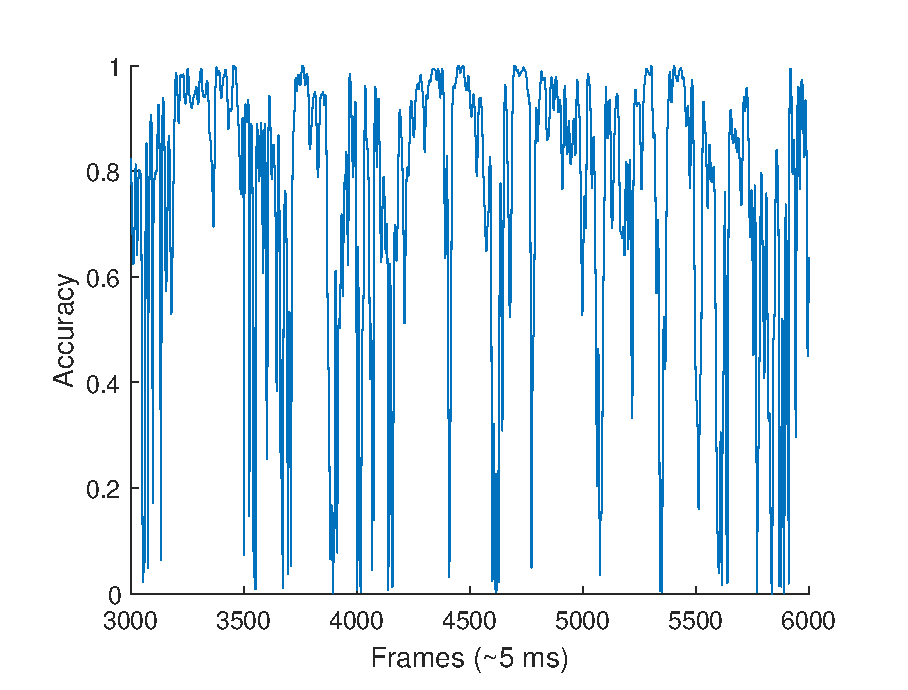
\includegraphics[width=0.48\linewidth]{images/matlab/accuracy_sig_20}
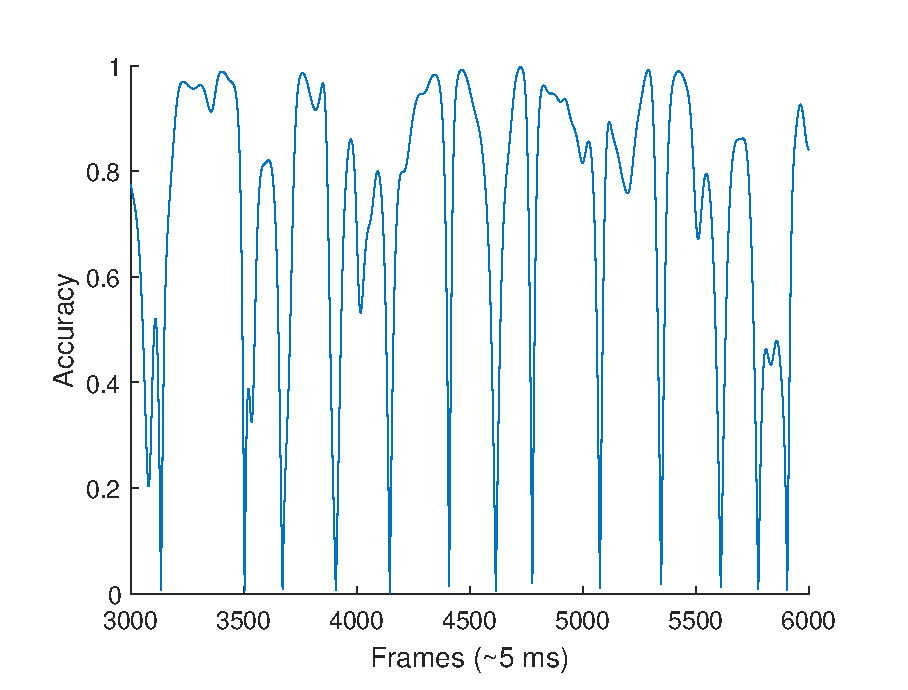
\includegraphics[width=0.48\linewidth]{images/matlab/accuracy_sig_100}
\caption{\textbf{Accuracy of the estimate over the duration of the experiment} - The accuracy corresponds to the absolute value of the dot product between both (normalized) direction of motion estimates (optic-flow sensor and motion capture system). The system displays regular drops in the accuracy of his estimate, which may be due to rapid changes in the motion of the camera.\label{fig:mocapAccuracy81}}
\end{figure}

\clearpage
\section{Conclusion}
In this report, we described a method for estimating the direction of motion based on high frequency and unscaled optic-flow measurements and its implementation on embedded hardware. With its low computational cost, at the expense of some minor approximations, this method enables the estimation of the direction of motion on hardware with limited resources. More importantly, as it relies on an iterative voting approach, this method exhibit high robustness to outliers and is easily scalable when it comes to finding a trade-off between accuracy and computational ovehead.

The efficiency of the method was first proven in simulation by synthetically generating optic-flow fields. The algorithm was also implemented on real hardware and assessed using a high precision motion capture system. Although the results show that improvements are required - such as adding further processing of the data (e.g. filtering, smoothing) - the method and its underlying approximations proved to be correct.

This method may benefit from an adapted size of the patch used by the Lucas-Kanade method depending on the distance to the center of camera. Moreover, the determination of the best estimate at each stage of the voting procedure may be improved using online clustering or averaging techniques so as to cope with competing bins. Similarly, we could consider refining the estimate from one frame to the other, building on the previous estimates or even other sensor measurements. Finally, besides improving the framework, the integration of the hardware on the drone would require the calibration of the camera frame with respect to the body frame of the robot. This latter procedure would typically entail the correlation (regression) of gyroscope measurements from the camera and the main board of the drone in order to estimation the transformation from one frame to the other. 

\bibliographystyle{ieeetr}
\bibliography{report}

\end{document}